% Options for packages loaded elsewhere
\PassOptionsToPackage{unicode}{hyperref}
\PassOptionsToPackage{hyphens}{url}
%
\documentclass[
]{book}
\usepackage{amsmath,amssymb}
\usepackage{lmodern}
\usepackage{iftex}
\ifPDFTeX
  \usepackage[T1]{fontenc}
  \usepackage[utf8]{inputenc}
  \usepackage{textcomp} % provide euro and other symbols
\else % if luatex or xetex
  \usepackage{unicode-math}
  \defaultfontfeatures{Scale=MatchLowercase}
  \defaultfontfeatures[\rmfamily]{Ligatures=TeX,Scale=1}
\fi
% Use upquote if available, for straight quotes in verbatim environments
\IfFileExists{upquote.sty}{\usepackage{upquote}}{}
\IfFileExists{microtype.sty}{% use microtype if available
  \usepackage[]{microtype}
  \UseMicrotypeSet[protrusion]{basicmath} % disable protrusion for tt fonts
}{}
\makeatletter
\@ifundefined{KOMAClassName}{% if non-KOMA class
  \IfFileExists{parskip.sty}{%
    \usepackage{parskip}
  }{% else
    \setlength{\parindent}{0pt}
    \setlength{\parskip}{6pt plus 2pt minus 1pt}}
}{% if KOMA class
  \KOMAoptions{parskip=half}}
\makeatother
\usepackage{xcolor}
\usepackage{longtable,booktabs,array}
\usepackage{calc} % for calculating minipage widths
% Correct order of tables after \paragraph or \subparagraph
\usepackage{etoolbox}
\makeatletter
\patchcmd\longtable{\par}{\if@noskipsec\mbox{}\fi\par}{}{}
\makeatother
% Allow footnotes in longtable head/foot
\IfFileExists{footnotehyper.sty}{\usepackage{footnotehyper}}{\usepackage{footnote}}
\makesavenoteenv{longtable}
\usepackage{graphicx}
\makeatletter
\def\maxwidth{\ifdim\Gin@nat@width>\linewidth\linewidth\else\Gin@nat@width\fi}
\def\maxheight{\ifdim\Gin@nat@height>\textheight\textheight\else\Gin@nat@height\fi}
\makeatother
% Scale images if necessary, so that they will not overflow the page
% margins by default, and it is still possible to overwrite the defaults
% using explicit options in \includegraphics[width, height, ...]{}
\setkeys{Gin}{width=\maxwidth,height=\maxheight,keepaspectratio}
% Set default figure placement to htbp
\makeatletter
\def\fps@figure{htbp}
\makeatother
\setlength{\emergencystretch}{3em} % prevent overfull lines
\providecommand{\tightlist}{%
  \setlength{\itemsep}{0pt}\setlength{\parskip}{0pt}}
\setcounter{secnumdepth}{5}
\usepackage{booktabs}
\ifLuaTeX
  \usepackage{selnolig}  % disable illegal ligatures
\fi
\usepackage[]{natbib}
\bibliographystyle{plainnat}
\IfFileExists{bookmark.sty}{\usepackage{bookmark}}{\usepackage{hyperref}}
\IfFileExists{xurl.sty}{\usepackage{xurl}}{} % add URL line breaks if available
\urlstyle{same} % disable monospaced font for URLs
\hypersetup{
  pdftitle={Draft Panduan Survei Keanekaragaman Hayati},
  pdfauthor={Biodive FFI`s IP},
  hidelinks,
  pdfcreator={LaTeX via pandoc}}

\title{Draft Panduan Survei Keanekaragaman Hayati}
\author{Biodive FFI`s IP}
\date{2022-09-02}

\begin{document}
\maketitle

{
\setcounter{tocdepth}{1}
\tableofcontents
}
\hypertarget{prakata}{%
\chapter*{Prakata}\label{prakata}}
\addcontentsline{toc}{chapter}{Prakata}

\textbf{Apa dan untuk siapa panduan ini?}

Panduan ini ditujukan bagi siapa saja yang berminat untuk melakukan survei keanekararagaman hayati (kehati) terutama bagi praktisi di ruang lingkup Fauna \& Flora International -- Indonesia Programme (FFI`s IP). Panduan ini disusun supaya pemantauan kehati dapat dilaksanakan dengan standar minimum yang sama, akurat dan dapat digunakan untuk pengambilan keputusan secara ilmiah.

Panduan ini dibuat sebagai ringkasan secara umum untuk melakukan pemantauan pada 4 taksa sebagai berikut; Avifauna, Herpetofauna, Mamalia serta Vegetasi yang berada dalam bioma terestrial. Panduan ini memiliki beberapa asumsi yang harus dipenuhi serta berbagai keterbatasan, disesuaikan dengan target dan luaran dari survei itu sendiri.

Kami menyadari bahwasannya metode pemantauan kehati selalu berkembang sehingga timbal balik dari pembaca diharapkan dapat terus menyempurnakan kebutuhan yang sesuai bagi para praktisi konservasi yang menggunakan panduan ini.

\hypertarget{pendahuluan}{%
\chapter*{Pendahuluan}\label{pendahuluan}}
\addcontentsline{toc}{chapter}{Pendahuluan}

Survei keanekaragaman hayati, bertujuan untuk mendapatkan informasi mengenai keberadaan satwa liar pada ruang dan waktu tertentu. Secara umum, survei kehati memiliki dua luaran yaitu;

\begin{enumerate}
\def\labelenumi{(\arabic{enumi})}
\item
  Inventarisasi, yang bertujuan untuk mendapatkan informasi mengenai fauna dan flora pada suatu area. Luarannya digunakan untuk membangun data dasar (baseline data). Biasanya, dalam kegiatan ini kita hanya membutuhkan konfirmasi apakah suatu spesies berhasil teridentifikasi di suatu area atau tidak.
\item
  Monitoring, yang dilakukan lebih dari satu kali dalam tahun atau musim yang berbeda untuk mendeteksi adanya perubahan (atau tidak ada perubahan) dalam suatu komunitas biologi. Monitoring juga digunakan untuk dapat melihat efek dari suatu kegiatan (contoh; {[}i{]} perambahan kawasan terhadap komunitas burung liar, {[}ii{]} pencemaran sungai terhadap mortalitas amfibi). Dalam monitoring, biasanya dibutuhkan penilaian kuantitatif yang kuat, daripada sekedar konfirmasi keberadaan spesies.
\end{enumerate}

Dalam kondisi aktual, sangat sulit untuk bisa mendapatkan nilai atau jumlah dari spesies yang seluruhnya menghuni suatu kawasan, terlebih di hutan tropis yang lebat dengan tingkat visibiltas yang rendah. Oleh karena itu, kita harus memiliki rancangan survei yang tepat, supaya mendapatkan sampel yang representatif dari kawasan tersebut \protect\hyperlink{rancangan-survei}{(Bab Rancangan Survei)}. Sindrom data ``\emph{sampah masuk, sampah keluar}'' juga berlaku untuk survei kehati. Jika kualitas data yang dikumpulkan lemah dan rancangan surveinya kurang menggambarkan areal terkait, maka akan sulit untuk menganalisa dan menginterpretasi data. Prosedur pengambilan sampel harus mengikuti protokol rancangan survei serta protokol pengambilan data dilapangan yang kuat, untuk memastikan pengumpulan data yang konsisten dengan kualitas semaksimal mungkin \protect\hyperlink{protokol-survei}{(Bab Prokotol Survei)}.

Menganalisa data merupakan bagian mendasar dari survei pada saat mempersiapkan rancangan survei, konsultasi dengan seorang ahli statistik satwa liar yang berpengalaman akan sangat bermanfaat untuk mempersiapkan analisa yang tepat \protect\hyperlink{analisa-data}{(Bab Analisa Data)}. Selain itu, luaran survei seringkali menjadi laporan kepada donor atau publikasi ilmiah sehingga data-data yang sudah didapatkan menjadi sangat berharga dan diperlukan untuk pengambilan keputusan yang tepat, serta memastikan data yang sudah didapat masih relevan untuk digunakan hingga bertahun-tahun kedepan. Oleh karena itu pengarsipan data juga bagian yang sangat penting, dan akan dibahas pada bagian pengelolaan data kehati \protect\hyperlink{pengelolaan-data}{(Bab Pengelolaan Data)}.

\hypertarget{pra-survei}{%
\chapter*{Pra-Survei}\label{pra-survei}}
\addcontentsline{toc}{chapter}{Pra-Survei}

\hypertarget{keahlian-dasar}{%
\section*{Keahlian Dasar}\label{keahlian-dasar}}
\addcontentsline{toc}{section}{Keahlian Dasar}

\hypertarget{keselamatan-kerja}{%
\section*{Keselamatan Kerja}\label{keselamatan-kerja}}
\addcontentsline{toc}{section}{Keselamatan Kerja}

Survei kehati seringkali dilakukan di daerah terisolir, jauh dari sarana umum dan kebutuhan akan bantuan medis profesional sulit dijangkau. Oleh karena itu penting untuk selalu sadar mengenai bahaya yang mengintai setiap saat, sehingga kita harus selalu waspada selama berkegiatan. Dibawah ini merupakan beberapa tips untuk dapat diikuti.

\textbf{Selalu bekerja bersama tim.} Jangan pernah melakukan pengamatan sendirian, pastikan minimal ada satu anggota lain yang ikut. Jika terjadi kecelakaan kerja, atau kondisi darurat, akan ada rekan kerja yang dapat memberikan pertolongan. Keberadaan rekan kerja juga mengurangi resiko tersesat saat pengamatan.

\textbf{Memberikan rencana perjalanan di luar tim.} Pastikan rekan kerja selain orang di luar tim survei, tahu rencana perjalanan dan kapan kalian akan kembali. Mereka dapat memberikan pertimbangan untuk melakukan evakuasi, jika kalian belum kembali dari waktu yang sudah direncakan. Rencana ini lebih baik jika ditulis detil hari per hari, sehingga mereka tahu perkiraan anda berada dimana pada suatu tanggal spesifik.

\textbf{Persiapkan peralatan keselamatan dengan seksama.} Pastikan membawa peta, kompas dan GPS jika ingin melakukan pengamatan di luar jalur. Membawa senter dan alat penerang jika estimasi perjalanan kalian hingga malam. Membawa peralatan pertolongan pertama jika berjalan jauh dari kamp utama. Membawa suplai makanan ekstra untuk melalui medan yang belum dikenal jika terdapat kelebihan hari.

\textbf{Persiapan untuk dapat memberikan pertolongan pertama.} Ada baiknya seluruh anggota tim, dilatih untuk dapat memberikan pertolongan pertama dengan benar dari pelaku medis profesional setempat (Dokter, petugas puskesmas, KSR PMI dll). Sehingga mereka sudah siap memberikan pertolongan kepada siapapun yang membutuhkan. Peralatan pertolongan pertama yang akan dibawa setidaknya mencakup; seperangkat peralatan penutup luka, tablet antibiotik, tablet malaria, bubuk rehidrasi, salep atau bedak anti jamur dan anti gatal, salep luka bakar dan \emph{snake bite-kit}.

\textbf{Persiapkan jalur evakuasi.} Persiapkan rute evakuasi, seperti titik evakuasi terdekat, kendaraan yang sudah siap sedia untuk menjemput tim yang perlu dievakuasi, sarana medis yang akan digunakan, protokol komunikasi dll.

\textbf{Menggunakan tenaga lokal.} Masyarakat lokal yang memiliki rutinitas berkegiatan di hutan dapat memberikan masukan mengenai jalur yang akan digunakan dan akan lebih waspada terhadap kondisi di kawasan tersebut (Potensi pohon tumbang, area rawan longsor dll).

\textbf{Hindari organisme dan area berbahaya.} Meskipun tujuan survei adalah untuk kajian jenis-jenis ular sekalipun, hindari menangkap ular berbisa. Jika kalian ragu apakah hewan tersebut berbahaya atau tidak sebaikmya tetap dihindari. Beberapa tumbuhan juga dapat menyebabkan gatal-gatal seperti jenis-jenis jelatang (Dendrocnide sp), beberapa lebah ada yang membuat sarang disemak-semak yang apabila tersentuh akan menyerang. Semakin sering ke lapangan anda akan dapat menghindari kejadian-kejadian tersebut. Hindari mandi di area sungai yang berpotensi dihuni oleh buaya. Jangan membuat kamp diarea yang terdapat pohon mati atau berpotensi rubuh.
Perhatikan penggunaan pisau tebas. Penggunaan pisau tebas saat membuka jalur seringkali melukai diri sendiri dan orang didekatnya. Selalu waspada dalam penggunaan pisau tebas, terlebih jika area yang dibuka merupakan semak-semak yang memiliki tingkat kekerasan dan kerapatan yang variatif.

\textbf{Kebersihan adalah prioritas.} Luka-luka kecil akibat duri atau gesekan kayu bisa memberikan infeksi jika tidak rutin dibersihkan dengan air dan sabun antiseptik. Kondisi dapur di area kamp juga harus diperhatikan, terkadang anggota tim membuang sampah organik sembarangan, hal ini dapat menyebabkan masalah pencernaan.

\textbf{TERPENTING. \emph{Use common sense!}.} Seringkali kecelekaan terjadi karena hal yang dari awal dapat dihindari seperti menyebrang sungai deras tanpa pengaman, memanjat pohon untuk mencari sinyal, tersesat karena panik, memanjat tebing terjal tanpa bantuan tali dan lain-lain. Selalu ketahui batas diri masing-masing, anggota tim yang lain mungkin dapat melompat diantara celah tebing dengan mudah, atau melewati tebing hanya dengan menyebrangi sebatang kayu yang dijadikan jembatan, namun anda belum tentu dapat melewatinya. Merupakan pilihan yang bijak untuk berpikir mengenai keselamatan diri dan membuat alternatif pilihan terhadap hambatan yang ditemui.

\hypertarget{pembuatan-transek}{%
\section*{Pembuatan Transek}\label{pembuatan-transek}}
\addcontentsline{toc}{section}{Pembuatan Transek}

\hypertarget{rancangan-survei}{%
\chapter*{Rancangan Survei}\label{rancangan-survei}}
\addcontentsline{toc}{chapter}{Rancangan Survei}

Beragam teknik dalam mencuplik satwa liar sudah banyak dibahas dalam berbagai panduan (Bookhout, 1994; Elzinga et al., 2009). Dalam panduan ini kami menyimpulkan sebagian yang sering dipergunakan dalam ruang lingkup kerja FFI`s IP. Secara umum teknik cuplik ini dibagi dalam dua hal dalam koleksi datanya, yaitu secara observatif atau perjumpaan langsung dan penangkapan. Konteks penangkapan dalam hal ini tidak hanya terbatas menangkap satwanya tapi juga dalam media gambar dan suara.

\hypertarget{protokol-survei}{%
\chapter*{Protokol Survei}\label{protokol-survei}}
\addcontentsline{toc}{chapter}{Protokol Survei}

\hypertarget{avifauna}{%
\section*{Avifauna}\label{avifauna}}
\addcontentsline{toc}{section}{Avifauna}

Pengamatan burung atau avifauna yang biasa dilakukan oleh FFI`s IP mengadopsi dua metode utama yaitu metode titik hitung di transek (\emph{Point transect}) (Buckland, 2006) dan daftar jenis MacKinnon (\emph{Mackinnon lists}) (MacKinnon \& Phillipps, 1993). Pada dasarnya metode point transect merupakan modifikasi dari metode titik hitung, namun unit sampelnya berada dalam transek yang sudah ditetapkan, metode ini efektif digunakan pada hutan tropis, dimana jalurnya seringkali sulit untuk dilalui dan burung menghuni seluruh strata hutan dari permukaan tanah hingga diatas tajuk. Dengan fokus pada titik tertentu di dalam transek, deteksi burung jadi lebih efektif. Pada Mackinnon lists survei dilakukan bisa di jalur transek atau pun di luar transek. Kedua metode ini saling melengkapi dalam pengumpulan data jenis-jenis burung

\hypertarget{persiapan-tim}{%
\subsection*{Persiapan Tim}\label{persiapan-tim}}
\addcontentsline{toc}{subsection}{Persiapan Tim}

Tim avifauna idealnya terdiri dari 2 orang, yaitu pengamat utama dan asisten lapangan. Dengan peran dan tanggung jawab yang terangkum dalam tabel \ref{tab:tbta}.

\begin{longtable}[]{@{}
  >{\raggedright\arraybackslash}p{(\columnwidth - 4\tabcolsep) * \real{0.1765}}
  >{\raggedright\arraybackslash}p{(\columnwidth - 4\tabcolsep) * \real{0.4118}}
  >{\raggedright\arraybackslash}p{(\columnwidth - 4\tabcolsep) * \real{0.4118}}@{}}
\caption{\label{tab:tbta} Peran dan tanggung jawab tim avifauna}\tabularnewline
\toprule()
\begin{minipage}[b]{\linewidth}\raggedright
Peran
\end{minipage} & \begin{minipage}[b]{\linewidth}\raggedright
Tanggung jawab
\end{minipage} & \begin{minipage}[b]{\linewidth}\raggedright
Syarat khusus
\end{minipage} \\
\midrule()
\endfirsthead
\toprule()
\begin{minipage}[b]{\linewidth}\raggedright
Peran
\end{minipage} & \begin{minipage}[b]{\linewidth}\raggedright
Tanggung jawab
\end{minipage} & \begin{minipage}[b]{\linewidth}\raggedright
Syarat khusus
\end{minipage} \\
\midrule()
\endhead
Pengamat utama & Mengamati dan mengidentifikasi burung pada lokasi yang disurvei, kemudian memberikan informasi pada pencatat mengenai data yang dibutuhkan seperti yang tertera pada lembar data & Memahami protokol serta identifikasi jenis burung dan penggunaan peralatan pendukung survei \\
Asisten lapangan & Mencatat data temuan survei dan juga sebagai pencatat waktu (\emph{time keeper}) & Memahami protokol survei avifauna dengan baik \\
\bottomrule()
\end{longtable}

\hypertarget{peralatan}{%
\subsection*{Peralatan}\label{peralatan}}
\addcontentsline{toc}{subsection}{Peralatan}

\begin{longtable}[]{@{}
  >{\raggedright\arraybackslash}p{(\columnwidth - 4\tabcolsep) * \real{0.1765}}
  >{\raggedright\arraybackslash}p{(\columnwidth - 4\tabcolsep) * \real{0.4118}}
  >{\raggedright\arraybackslash}p{(\columnwidth - 4\tabcolsep) * \real{0.4118}}@{}}
\caption{\label{tab:tbpa} Peralatan yang dibutuhkan tim avifauna}\tabularnewline
\toprule()
\begin{minipage}[b]{\linewidth}\raggedright
Peralatan
\end{minipage} & \begin{minipage}[b]{\linewidth}\raggedright
Penggunaan
\end{minipage} & \begin{minipage}[b]{\linewidth}\raggedright
Spesifikasi
\end{minipage} \\
\midrule()
\endfirsthead
\toprule()
\begin{minipage}[b]{\linewidth}\raggedright
Peralatan
\end{minipage} & \begin{minipage}[b]{\linewidth}\raggedright
Penggunaan
\end{minipage} & \begin{minipage}[b]{\linewidth}\raggedright
Spesifikasi
\end{minipage} \\
\midrule()
\endhead
Alat Tulis & Pencatatan data dan penandaan & Kuat, tidak mudah luntur \\
Lembar data & Lembar pencatatan data & Tahan air \\
Alat Navigasi (GPS, Peta dan Kompas) & Untuk navigasi sekaligus penanda lokasi geografis & Tahan air \\
Binokuler & Untuk melihat dan mengidentifikasi burung & Perbesaran lensa minimal 8 x 40 atau 7 x 50 \\
Kamera & Untuk dokumentasi burung dan identifikasi lebih lanjut & DSLR dengan lensa tele 300 -- 400 mm. Alternatif lainnya dapat menggunakan kamera digital \emph{prosummer} dengan perbesaran optik diatas 30x \\
Perekam suara genggam & Merekam suara burung untuk identifikasi lebih lanjut & Perekam suara digital dengan fitur \emph{directional microphone} \\
Perekam suara pasif & Merekam suara burung untuk identifikasi burung yang sensitif & Tahan air. Perangkat yang biasa digunkan adalah \emph{audiomoth} (Hill et al., 2019) \\
\bottomrule()
\end{longtable}

\hypertarget{protokol-pengamatan}{%
\subsection*{Protokol Pengamatan}\label{protokol-pengamatan}}
\addcontentsline{toc}{subsection}{Protokol Pengamatan}

\hypertarget{titik-hitung}{%
\subsubsection*{Titik hitung}\label{titik-hitung}}
\addcontentsline{toc}{subsubsection}{Titik hitung}

Protokol untuk survei dengan metode titik hitung dalam transek yang dilakukan oleh FFI`s IP menggunakan enam buah titik hitung dengan rentang antar titik berjarak 200m sehingga akan membentuk garis transek sejauh 1 Km (Gambar \ref{fig:figpc}). Radius pengamatan per titik adalah 50m dari titik pusat. Titik pusat yang dimaksud adalah titik yang telah ditentukan. Pengamatan menggunakan titik hitung mengikuti asumsi-asumsi berikut ini:

\begin{enumerate}
\def\labelenumi{\arabic{enumi}.}
\tightlist
\item
  Burung tidak mendekati pengamat atau terbang;
\item
  Burung yang ada dalam titik cuplik dapat terdeteksi 100\%;
\item
  Burung tidak bergerak selama perhitungan;
\item
  Burung berperilaku bebas (tidak tergantung satu sama lain);
\item
  Pelanggaran terhadap asumsi tersebut tidak berpengaruh terhadap habitat atau desain studi;
\item
  Estimasi jarak akurat;
\item
  Burung dapat teridentifikasi dengan baik seluruhnya.
\end{enumerate}

Dalam pelaksanaannya, pengamat berhenti pada suatu titik pengamatan selama 20 menit untuk mengamati dan mencatat jenis burung yang dapat diidentifikasi di sekitar lokasi penelitian. Setelah 20 menit, pengamat kemudian berpindah ke titik pengamatan lain dan kemudian melakukan pengamatan lagi di titik pengamatan tersebut dengan waktu yang sama yaitu selama 20 menit. Jumlah titik pada setiap jalur adalah enam titik, dengan jarak masing-masing titik 200 m, sehingga panjang jalur pengamatannya adalah 1 km. Pengamatan dilakukan pada pagi hari pukul 06.00-09.00 WIB dan sore hari pukul 15.30-18.00 WIB. Perjumpaan terhadap jenis burung di luar titik pengamatan tidak diperhitungkan. Pada setiap jalur pengamatan dilakukan pengulangan pengamatan sebanyak dua kali. Pengamatan dilakukan melalui perjumpaan langsung dengan objek (visual) dan melalui suara. Parameter yang dicatat adalah jenis burung, jumlah yang ditemukan dan aktifitas. Jika memungkinkan, maka jarak setiap burung yang dijumpai terhadap pengamat juga diukur, dengan data seperti itu maka kepadatan burung juga dapat dihitung dengan konsep distance sampling (Buckland et al., 2015).

\begin{figure}

{\centering 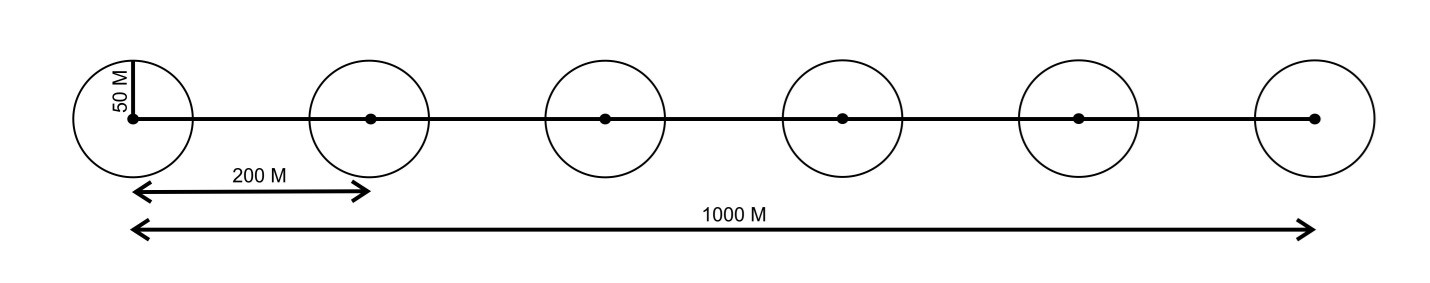
\includegraphics[width=1\linewidth]{images/pc_ilustration} 

}

\caption{Ilustrasi titik hitung di transek}\label{fig:figpc}
\end{figure}

\textbf{Cara Pelaksanaan :}
1. Sebelum menuju ke titik hitung, pengamat sudah menentukan lokasi titik -- titik hitung tersebut di GPS.
2. Pengamat menuju titik yang sudah ditentukan di dalam transek, dimana jarak antar point sepanjang 200 meter.
3. Setiap titik ditandai di dalam GPS
4. Pengamat berdiri di titik tengah dari point yang sudah ditentukan.
5. Pengamat mengamati dan mencatat burung yang terdengar ataupun terlihat selama 20 menit ke dalam lembar pengamatan titik hitung (Gambar \ref{fig:ldpth})
6. Untuk penggunaan perekam suara, bisa digunakan selama 20 menit pengamatan atau ketika mendengar suara-suara yang menarik.
7. Asisten dapat membantu mengukur parameter lingkungan disekitar lokasi pengamatan selama durasi pengamatan kedalam lembar data parameter lingkungan (Gambar \ref{fig:ldppl}) secara semi-kuantitatif.

\hypertarget{daftar-jenis-mackinnon}{%
\subsubsection*{Daftar jenis MacKinnon}\label{daftar-jenis-mackinnon}}
\addcontentsline{toc}{subsubsection}{Daftar jenis MacKinnon}

Metode ini pada dasarnya membuat sejumlah daftar yang berisi catatan nama jenis-jenis burung yang dijumpai untuk mendapat gambaran cepat mengenai kekayaan dan komposisi jenis burung pada suatu wilayah. Rincian prosedur penyusunan daftar dijelaskan di bawah ini.

\textbf{Cara Pelaksanaan:}
1. Berjalan di suatu habitat, seperti perjalanan dari desa menuju camp, di sekitar camp, dari camp menuju transek, transek satu kilo diluar point dan ketika perjalanan dari point menuju point yang lain dan mencatat semua jenis burung yang dijumpai sampai tercatat 20 jenis burung dalam satu daftar. Satu jenis burung hanya dicatat satu kali saja dalam satu daftar ini, meskipun dijumpai beberapa kali

\begin{enumerate}
\def\labelenumi{\arabic{enumi}.}
\setcounter{enumi}{1}
\item
  Setelah tercatat 20 jenis burung, lalu membuat daftar yang baru untuk mencatat jenis-jenis yang dijumpai selanjutnya (daftar no.2). Apabila dijumpai jenis yang pernah tercatat dalam daftar pertama maka tetap dicatat dalam daftar kedua, tetapi sebagaimana dalam pembuatan daftar pertama, jenis yang sudah dicatat dalam daftar kedua tidak boleh dicatat lagi meskipun dijumpai beberapa kali (di dalam satu daftar tidak boleh ada pengulangan jenis). Jika suatu spesies ditemukan kembali dalam 1 daftar yang belum mencapai 20 spesies, maka spesies tersebut hanya dihitung sebagai tambahan populasi pada spesies yang sama (bukan spesies baru)
\item
  Jika menemukan spesies yang menarik maka di tandai posisinya di dalam GPS, begitu juga jika mendengar suara yang menarik maka bisa di rekam di perekam suara.
\end{enumerate}

Metode ini meskipin sederhana, namun membutuhkan pengetahuan yang baik terhadap ekologi dan perilaku burung-burung di area survei. Terkadang pengamat boleh untuk duduk bersembunyi sebentar saat berada habitat yang sedang berbuah dan berbunga untuk melihat dan mendengar burung-burung yang berkunjung. Lampiran Gambar \ref{fig:ldpml}, merupakan contoh lembar data untuk metode daftar jenis MacKinnon.

\hypertarget{perekam-suara-pasif}{%
\subsubsection*{Perekam suara pasif}\label{perekam-suara-pasif}}
\addcontentsline{toc}{subsubsection}{Perekam suara pasif}

Untuk melengkapi daftar jenis burung-burung yang mungkin terlalu sensitif terhadap keberadaan manusia / pengamat, maka penggunaan perekam suara dapat dijadikan alternatif karena mampu merekam tanpa kehadiran pengamat selama waktu yang dibutuhkan dan tidak akan ada bias dalam identifikasi karena memiliki data suara yang terdokumentasikan dengan baik. Dalam praktiknya, FFI`s IP seringkali menggunakan perangkat perekam suara \emph{audiomoth} untuk merekam suara burung-burung di hutan.

Perekam suara dapat ditempatkan disetiap titik hitung sebagai data pelengkap atau lokasi spesifik lainnya yang diperkirakan memiliki kelimpahan burung dengan jarak minimal antar perekam suara 250 - 1000 meter. Setiap perekam suara diaktifkan minimal 1 x 24 jam agar burung diurnal dan nokturnal dapat terekam. Prinsipnya semakin lama di aktifkan maka data yang diperoleh semakin baik, perangkat ini dapat diaktifkan hingga sekitar 10 hari dengan baterai tipe alkalin dengan pengaturan 5 menit merekam dan 30 menit jeda. Adapun protokol penggunaan perekam suara adalah sebagai berikut;

\begin{enumerate}
\def\labelenumi{\arabic{enumi}.}
\item
  Melakukan pengaturan perangkat dengan spesifikasi sebagai berikut

  \begin{itemize}
  \tightlist
  \item
    Sample rate; 48 Khz
  \item
    Gain; Medium
  \item
    Sleep duration; 1800s
  \item
    Recording duration; 300s
  \end{itemize}
\item
  Pastikan pengaturan sudah sesuai dengan yang kita inginkan, dengan melakukan simulasi terlebih dahulu
\item
  Beri label pada setiap perangkat untuk membedakan antar perekam suara
\item
  Bungkus perangkat dengan plastik atau penutup kedap air dan pasang pada batang pohon dengan ketinggian sekitar 2 meter.
\item
  Catat kordinat pemasangan, waktu mulai dan waktu berakhirnya pada lembar pengamatan
\end{enumerate}

\hypertarget{herpetofauna}{%
\section*{Herpetofauna}\label{herpetofauna}}
\addcontentsline{toc}{section}{Herpetofauna}

Survei herpetofauna biasanya didasarkan pada tujuan untuk mendapatkan informasi mengenai:

\begin{enumerate}
\def\labelenumi{\arabic{enumi}.}
\tightlist
\item
  Daftar jenis herpetofauna pada suatu lokasi
\item
  Densitas atau kelimpahan relatif pada suatu lokasi
\item
  Penyebaran jenis
\item
  Aspek spesifik pada satu jenis seperti penggunaan habitat, pola aktifitas, biologi, reproduksi, dan sebagainya
\end{enumerate}

Perbedaan tujuan survei berpengaruh terhadap metode yang digunakan, usaha (effort), biaya dan waktu. Untuk survei yang bertujuan memperoleh daftar jenis, untuk memperoleh sebanyak mungkin jenis pada suatu lokasi perlu dilakukan pencarian aktif dan jebakan (pasif) dengan waktu yang mencakup siang dan malam hari. Hasil survei juga tergantung pada kondisi cuaca dan musim. Terdapat beberapa kendala dalam survei daftar jenis, diantaranya lama pengamatan yang mempengaruhi hasil temuan, biaya dan efektifitas kerja. Perbandingan hasil survei baik pada lokasi yang sama ataupun berbeda, perlu memperhatikan usaha (effort), musim dilakukan survei, dan metode yang digunakan

Metode yang biasa digunakan oleh FFI`s IP adalah pencarian langsung dengan metode Survei Perjumpaan Visual (Visual Encounter surveis - VES) (Gambar \ref{fig:figves}). Metode ini dilakukan dengan menyusuri area atau habitat herpetofauna dengan batasan waktu tertentu. Pencarian herpetofauna difokuskan pada tipe jenisnya, pencarian di tajuk pohon, batang dan ranting untuk jenis arboreal, kemudian pencarian di balik serasah, batu, kayu lapuk untuk jenis terestrial, terdapat juga jenis yang hidup di dalam tanah (fosorial) dan perairan seperti sungai, danau, dan kolam.

Metode VES memiliki batasan waktu pencarian di luar waktu penangkapan dan pencatatan. Penentuan batas waktu total biasanya 2 jam per orang per pengambilan sampel. Metode ini dapat dilakukan pada jalur transek, plot petak, aliran sungai, kolam dan lainya. Metode diterapkan dengan melakukan survei lokasi pengamatan dengan menentukan lokasi pengamatan yang memiliki dugaan habitat herpetofauna, membuat sedikit jalur untuk memudahkan pengamatan malam hari dan memberi tanda pada lokasi. Data yang dikumpulkan adalah ukuran lokasi, karakteristik habitat berupa vegetasi dominan, kerapatan tajuk, kondisi fisik lokasi dan dokumentasi lokasi.

\begin{figure}

{\centering 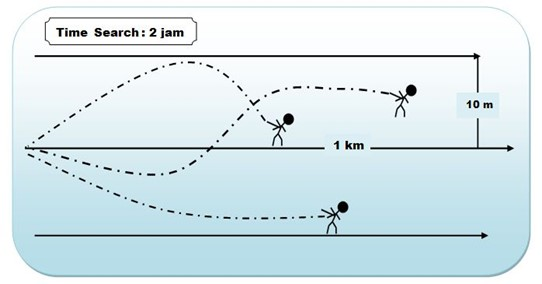
\includegraphics[width=1\linewidth]{images/ves_ilustration} 

}

\caption{Desain VES dalam transek dengan panjang 1 km dan lebar kiri – kanan transek adalah 5 - 10 m.}\label{fig:figves}
\end{figure}

\textbf{Persiapan}
Langkah awal sebelum melakukan survei salah satunya adalah pengumpulan informasi terkait lokasi survei dan data dasar pada lokasi. Informasi lokasi survei yang dimaksud antara lain, status administrasi, letak dan aksesibilitas lokasi survei. Sedangkan informasi data dasar berupa peta lokasi, data hasil survei sebelumnya dan data pendukung lain yang diperlukan. Informasi tersebut dapat diperoleh secara langsung kepada pengelola lokasi survei atau melalu lembaga yang menyediakan informasi terkait.

\hypertarget{persiapan-tim-1}{%
\subsection*{Persiapan Tim}\label{persiapan-tim-1}}
\addcontentsline{toc}{subsection}{Persiapan Tim}

Tim herpetofauna idealnya terdiri dari 3 orang, yaitu seorang pencatat, pencari atau pengamat, dan asisten lapangan (Tabel \ref{tab:tabtmh}). Namun pada kondisi tertentu, survei dapat dilakukan oleh 2 orang saja dengan konsekuensi seorang pencatat berperan juga menjadi spotter pada saat yang sama.

\begin{longtable}[]{@{}
  >{\raggedright\arraybackslash}p{(\columnwidth - 4\tabcolsep) * \real{0.1765}}
  >{\raggedright\arraybackslash}p{(\columnwidth - 4\tabcolsep) * \real{0.4118}}
  >{\raggedright\arraybackslash}p{(\columnwidth - 4\tabcolsep) * \real{0.4118}}@{}}
\caption{\label{tab:tabtmh} Peran dan tanggung jawab tim herpetofauna}\tabularnewline
\toprule()
\begin{minipage}[b]{\linewidth}\raggedright
Peran
\end{minipage} & \begin{minipage}[b]{\linewidth}\raggedright
Tanggung jawab
\end{minipage} & \begin{minipage}[b]{\linewidth}\raggedright
Syarat khusus
\end{minipage} \\
\midrule()
\endfirsthead
\toprule()
\begin{minipage}[b]{\linewidth}\raggedright
Peran
\end{minipage} & \begin{minipage}[b]{\linewidth}\raggedright
Tanggung jawab
\end{minipage} & \begin{minipage}[b]{\linewidth}\raggedright
Syarat khusus
\end{minipage} \\
\midrule()
\endhead
Peneliti utama; Pengamat (\emph{Spotter}) & Mencari herpetofauna pada lokasi yang disurvei, mengambil foto dari individu herpetofauna, kemudian memberikan informasi pada pencatat mengenai data yang dibutuhkan seperti yang tertera pada lembar data & Memahami protokol serta identifikasi jenis dan penggunaan peralatan pendukung survei \\
Asisten I: Pencatat & Mencatat data temuan survei dan juga sebagai pencatat waktu (\emph{time keeper}) & Memahami protokol survei herpetofauna dengan baik \\
Asisten II: Penunjuk jalan & Porter atau penunjuk jalan saat survei dan membantu pencarian herpetofauna & Memahami area survei dan kemampuan membaca jalur \\
\bottomrule()
\end{longtable}

\hypertarget{peralatan-1}{%
\subsection*{Peralatan}\label{peralatan-1}}
\addcontentsline{toc}{subsection}{Peralatan}

Peralatan survei yang dipersiapkan disesuaikan dengan waktu, metode dan jumlah surveior. Menyusun daftar peralatan perlu pengelompokan sesuai fungsi untuk mempermudah persiapan, secara umum disusun sebagai berikut:

\begin{longtable}[]{@{}
  >{\raggedright\arraybackslash}p{(\columnwidth - 2\tabcolsep) * \real{0.3000}}
  >{\raggedright\arraybackslash}p{(\columnwidth - 2\tabcolsep) * \real{0.7000}}@{}}
\caption{\label{tab:tbph} Peralatan yang dibutuhkan tim herpetofauna}\tabularnewline
\toprule()
\begin{minipage}[b]{\linewidth}\raggedright
Kelompok
\end{minipage} & \begin{minipage}[b]{\linewidth}\raggedright
Alat
\end{minipage} \\
\midrule()
\endfirsthead
\toprule()
\begin{minipage}[b]{\linewidth}\raggedright
Kelompok
\end{minipage} & \begin{minipage}[b]{\linewidth}\raggedright
Alat
\end{minipage} \\
\midrule()
\endhead
Navigasi & GPS, kompas, dan peta \\
Survei dan koleksi data & Senter kepala (\emph{headlamp}), jam tangan, penggaris, meteran, plastik sampel, kantong kain, kamera, alat tulis, lembar data, Sepatu boot \\
Preservasi & Kotak specimen, kain kasa, syringe, alat bedah, kertas label, benang, gunting, alkohol, formalin, toples spesimen \\
\bottomrule()
\end{longtable}

\textbf{Baterai}
Alat-alat seperti \emph{headlamp}, GPS dan Kamera. Kalkulasikan kebutuhan baterai tersebut sebelum melakukan survei. Informasi lama daya tahan baterai saat digunakan oleh suatu alat sangat penting untuk menghitung berapa banyak jumlah baterai yang digunakan setiap harinya.

Tipe baterai yang digunakan perlu menjadi perhatian. Disarankan menggunakan baterai yang memiliki ketahanan yang lama seperti baterai alkaline \emph{non-rechargeable}. Hal tersebut berdasarkan pada pertimbangan biasanya tidak terdapat sumber listrik pada lokasi survei.

Selain peralatan survei, perlu dipersiapkan perlengkapan pribadi untuk kegiatan di lapangan, logistik bahan lapang, makanan dan obat-obatan. Kegiatan di lapangan sebaiknya disusun dengan jadwal kegiatan perhari dan tabel waktu selama survei agar efektif.

\hypertarget{protokol-pengamatan-1}{%
\subsection*{Protokol Pengamatan}\label{protokol-pengamatan-1}}
\addcontentsline{toc}{subsection}{Protokol Pengamatan}

\hypertarget{waktu-pengamatan}{%
\subsubsection*{Waktu Pengamatan}\label{waktu-pengamatan}}
\addcontentsline{toc}{subsubsection}{Waktu Pengamatan}

Pengamatan pada waktu siang hari dilakukan dengan estimasi waktu pukul 08.00 -- 10.00 untuk mencari jenis yang aktif pada siang hari (diurnal), terutama untuk kelompok reptil (kadal, ular). Pengamatan pada waktu malam hari dilakukan dengan estimasi waktu pukul 19.00 -- 22.00 pada lokasi yang telah disurvei saat siang hari. Tidak ada batasan berapa jumlah pengamat pada tiap pengamatan, namun demi keamanan minimal jumlah pengamat adalah 2 orang

\hypertarget{persiapan-pengamatan}{%
\subsubsection*{Persiapan Pengamatan}\label{persiapan-pengamatan}}
\addcontentsline{toc}{subsubsection}{Persiapan Pengamatan}

\begin{itemize}
\tightlist
\item
  Persiapkan alat yang diperlukan dan lakukan pengecekan kondisinya. Terutama GPS, \emph{headlamp} dan kamera serta persiapkan baterai cadangannya.
\item
  Cek kesehatan anggota tim
\item
  Lakukan pembagian tugas. Pembagian tugas yang dimaksud adalah pembagian kerja kepada tiap anggota tim berupa pencari / pengamat utama, dokumentasi, pengukur dan pencatat data.
\item
  Cek kembali kondisi alat -- alat sesampainya di lokasi observasi yang telah ditentukan dan sesaat sebelum melakukan pengamatan
\end{itemize}

\hypertarget{koleksi-data}{%
\subsubsection*{Koleksi Data}\label{koleksi-data}}
\addcontentsline{toc}{subsubsection}{Koleksi Data}

\begin{itemize}
\tightlist
\item
  Hal pertama yang dilakukan adalah pencatatan waktu, kondisi cuaca dan lingkungan (suhu dan kelembapan udara).
\item
  Mulai mencari dengan berjalan perlahan sambil menyorotkan lampu pada pada substrat tajuk, batang, serasah, lubang, di balik batu dan kayu mati. Indikasi adanya herpetofauna dapat dilihat dengan pantulan cahaya dari mata satwa tersebut. Terkadang dapat diketahui melalui suara, terutama untuk katak dan kodok.
\item
  Saat menemukan satwa, hal pertama yang dicatat adalah waktu ditemukan, tempat ditemukan (jarak horizontal dari badan air, jarak vertical dari permukaan tanah), substrat, aktifitas, dan nama jenis jika sudah dapat diketahui pada tally sheet
\item
  Tangkap satwa tersebut jika kondisi memungkinkan untuk dilakukan.

  \begin{itemize}
  \tightlist
  \item
    Katak: Perlahan dekati satwa hingga mencapai jangkauan tangan, posisikan tangan sejajar dengan badan katak dari belakang. Cekungkan tangan dan arahkan ke depan moncong katak dengan perlahan, kemudian dengan gerakan cepat menangkap katak dengan genggaman yang tidak terlalu kuat
  \item
    Ular: Jangan coba untuk menangkap ular jika tidak benar -- benar diketahui bahwa ular tesebut tidak berbisa. Gunakan graber atau tongkat untuk mengangkat ular kemudian letakkan di atas permukaan tanah. Perlahan tahan kepala ular dengan tongkat. Setelah tenang, genggam leher ular dengan posisi semua jari berada di bagian leher dan jempol menahan bagian atas kepala. Jangan mengambil risiko untuk menangkap ular berbisa seperti spesies--spesies dari famili Elapidae dan Viperidae. Cukup lakukan pengambilan foto dari beberapa bagian tubuh seperti punggung, sisi tubuh dan bagian atas, sisi kepala dari jarak yang relatif aman tanpa mengganggunya. Foto tersebut dapat dijadikan dokumentasi untuk keperluan identifikasi kemudian.\\
  \end{itemize}
\item
  Lakukan identifikasi jenis, ukur panjang badan (SVL) dan panjang ekor (Gambar \ref{fig:figmhf}. Untuk ular, gunakan graber atau tongkat untuk mengangkat ular kemudian letakkan di atas permukaan tanah. Perlahan tahan kepala ular dengan tongkat. Setelah tenang, genggam leher ular dengan posisi semua jari berada di bagian leher dan jempol menahan bagian atas kepala. Pengukuran panjang sebaiknya dilakukan dengan tetap meletakkan badan ular di atas tanah, sedangkan pengukuran menggunakan tali atau meteran jahit dengan mengikuti alur badan ular
\item
  Jika sudah dapat memastikan jenisnya dan selesai melakukan pengukuran, lepas kembali hewan tersebut ke tempat semula ditemukan.
\item
  Jika belum dapat teridentifikasi, masukkan hewan ke dalam plastik spesimen (untuk katak dan kodok), dan kantung kain (untuk reptil). Tulis kode jenis pada plastik dengan menggunakan spidol dengan tinta permanen (spidol waterproof), (catatan: satu plastik untuk satu individu), catat kode jenis di plastik pada tally sheet, dengan plastik spesimen. Catatan: jangan meniup plastik untuk memberikan udara.
\item
  Hentikan pengamatan saat:

  \begin{itemize}
  \tightlist
  \item
    Waktu pengamatan berakhir. Catat waktu akhir pengamatan, cuaca, dan kondisi lingkungan (suhu, kelembapan)
  \item
    Terjadi hujan lebat yang tidak memungkinkan pengamatan dilakukan, karena akan membahayakan pengamat saat melakukan pengamatan di sungai.
  \end{itemize}
\item
  Cek kembali kelengkapan alat, kondisi anggota tim dan sampel yang dibawa sebelum pulang.
\end{itemize}

\begin{figure}

{\centering 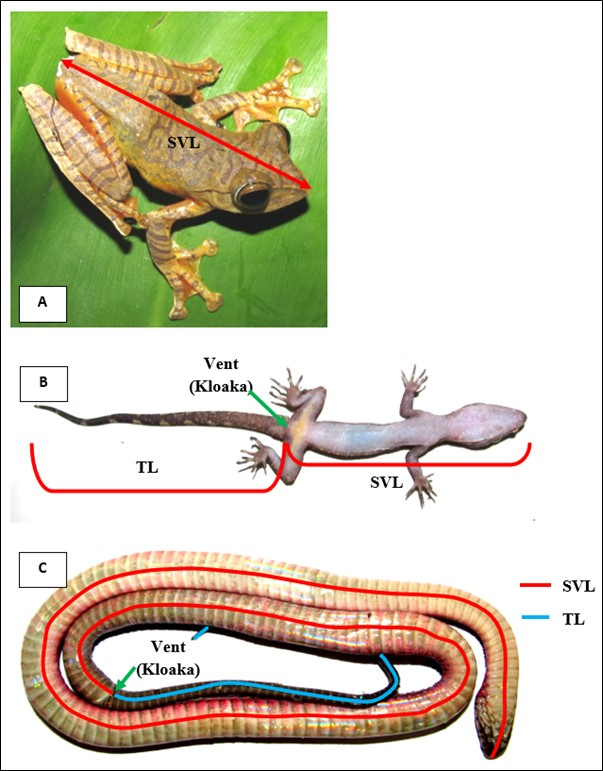
\includegraphics[width=1\linewidth]{images/mhf_ilustration} 

}

\caption{Pengukuran Snout Vent Length (SVL) dan Tail Length (TL) pada spesimen herpetofauna; A) Katak B) Kadal, Cicak, Biawak C) Ular}\label{fig:figmhf}
\end{figure}

Beberapa hal penting yang perlu diperhatikan dalam melakukan survei Herpetofauna, adalah sebagai berikut:

\begin{itemize}
\tightlist
\item
  Pengamatan dilakukan pada lokasi yang telah disurvei dengan data jalur, koordinat lokasi, penanda jalur yang lengkap dan perizinan kepada pengelola serta masyarakat sekitar lokasi.
\item
  Surveior minimal dua orang, sebaiknya didampingi oleh pemandu yang mengetahui kondisi lokasi dan mampu melakukan pengamatan malam.
\item
  Persiapkan perlengkapan lapang, alat komunikasi dan perlengkapan P3K untuk mengantisipasi terjebak di lokasi pengamatan dan terpaksa menginap.
\item
  Pertimbangkan kondisi cuaca dan kesehatan tim, jika tidak memungkinkan jangan dipaksakan untuk melakukan pengamatan.
\item
  Surveior sebaiknya melakukan pencarian dengan jarak yang dapat dipantau satu dengan yang lainnya.
\item
  Saat ditemukan satwa, sesegera mungkin mengambil data yang diperlukan dan melanjutkan pencarian.
\item
  Perlakukan satwa yang ditangkap dengan hati-hati tanpa menyakiti, lebih baik menggunakan tangan secara langsung untuk memegang satwa.
\item
  Penanganan pada jenis yang berbahaya dan sulit ditangkap sebaiknya dilakukan minimal dua orang.
\item
  Penyimpanan spesimen yang ditangkap, untuk amfibi ditempatkan pada plastik, sedangkan untuk reptil ditempatkan pada kantong kain dan satu individu satu kantong.
\item
  Pengamatan selesai jika jalur atau plot yang ditentukan sudah teramati, alokasi waktu sudah habis, perubahan kondisi cuaca dan medan yang membahayakan.
\item
  Secepat mungkin dilakukan pengambilan data pada spesimen yang ditangkap dan sesegera mungkin dilakukan preservasi/ pengawetan jika diperlukan.
\item
  Lakukan preservasi pada lokasi yang terpisah, bersih, gunakan masker dan sarung tangan karet (\emph{latex gloves}) dan jangan lupa mencuci tangan sebelum dan sesudah preservasi.
\item
  Penyimpanan spesimen yang diawetkan sebaiknya diletakkan pada tempat khusus yang terhindar dari cahaya matahari langsung.
\end{itemize}

\hypertarget{mamalia}{%
\section*{Mamalia}\label{mamalia}}
\addcontentsline{toc}{section}{Mamalia}

\hypertarget{persiapan-tim-2}{%
\subsection*{Persiapan Tim}\label{persiapan-tim-2}}
\addcontentsline{toc}{subsection}{Persiapan Tim}

\hypertarget{peralatan-2}{%
\subsection*{Peralatan}\label{peralatan-2}}
\addcontentsline{toc}{subsection}{Peralatan}

\hypertarget{protokol-pengamatan-2}{%
\subsection*{Protokol Pengamatan}\label{protokol-pengamatan-2}}
\addcontentsline{toc}{subsection}{Protokol Pengamatan}

\hypertarget{vegetasi}{%
\section*{Vegetasi}\label{vegetasi}}
\addcontentsline{toc}{section}{Vegetasi}

Secara umum, survei vegetasi dan pengukuran biomassa yang dilakukan FFI`s IP bertujuan untuk menggambarkan kondisi hutan melalui analisis vegetasi (jenis tumbuhan dominan, kerapatan pohon, tutupan kanopi pohon, dsb) serta potensi cadangan karbon yang terkandung di hutan tersebut (karbon atas permukaan, bawah permukaan, serasah, dan pohon mati). Analisis vegetasi biasanya digunakan untuk menggambarkan struktur dan komposisi dari vegetasi suatu habitat. Selain itu, sekaligus juga dapat digunakan untuk inventarisasi biodiversitas floristik suatu area.

Dari hasil survei vegetasi, kandungan karbon (karbon permukaan dan bawah) dapat di estimasi dengan menggunakan persamaan alometrik yang paling sesuai (Krisnawati et al., 2012; SNI 7724:2011; SNI 7725:2011). Persamaan alometrik yang digunakan akan menggambarkan biomassa dari tiap jenis pohon yang di data. Biomassa tersebut kemudian dikalikan dengan faktor pengali standar, 47\% (IPCC, 2012), untuk memperoleh kandungan karbon dari tiap jenis pohon yang di data. Kandungan karbon tersebut kemudian dikalikan dengan berat molekul CO2 (3.67) untuk menghasilkan potensi emisi CO2 dari tiap jenis pohon yang di data. Pertumbuhan pohon atau riap dapat dihitung dengan menggunakan data lokal dari plot permanen, atau menggunakan asumsi pertumbuhan sebesar 3,4-ton biomassa per hektar per tahun (Eggleston et al., 2006; Penman et al., 2003).

\textbf{Batasan Studi}

survei vegetasi yang dilakukan FFI`s IP dibatasi pada tingkat tumbuhan tinggi tegakan kayu dengan ukuran kayu yang diukur dimulai dari diameter setinggi dada (DBH) 5 cm, dan diklasifikasikan ke dalam 3 kelas, yaitu:

\begin{itemize}
\tightlist
\item
  Kelas C: Tiang dan pancang, DBH 5 -- 14,99 cm
\item
  Kelas B: Pohon sedang, DBH 15 -- 29,99 cm
\item
  Kelas A: Pohon besar, DBH ≥ 30 cm
\end{itemize}

Liana dan pohon perambat tidak masuk dalam kategori di atas karena tidak berbentuk tegakan. Pembatasan ini dilakukan untuk menyesuaikan efektifitas usaha dan waktu dimana sedapat mungkin objek yang disurvei merupakan komunitas atau struktur utama pembentuk vegetasi. Selain itu, data pengukuran botani ini digunakan pula untuk penghitungan karbon tegakan (Above Ground Biomass - AGB) dimana kandungan karbon terbesar berada pada ketiga kelas kayu tersebut. Karbon pada tingkat semaian dan herba tidak berpengaruh secara signifikan terhadap nilai cadangan karbon

\hypertarget{persiapan-tim-3}{%
\subsection*{Persiapan Tim}\label{persiapan-tim-3}}
\addcontentsline{toc}{subsection}{Persiapan Tim}

Pelaksanaan survei vegetasi di FFI`s IP membutuhkan ketelitian dan langkah kerja yang cukup banyak sehingga membutuhkan beberapa asisten untuk membantu di lapangan. Idealnya, satu orang peneliti utama dibantu dengan 4 orang asisten lokal dengan peran dan tanggung jawab seperti terlihat pada Tabel \ref{tab:tabtmv}. Dalam pelaksanaannya, jumlah, susunan dan formasi peran dan tanggung jawab asisten lokal dapat berubah sesuai kondisi.

\begin{longtable}[]{@{}
  >{\raggedright\arraybackslash}p{(\columnwidth - 4\tabcolsep) * \real{0.2941}}
  >{\raggedright\arraybackslash}p{(\columnwidth - 4\tabcolsep) * \real{0.4118}}
  >{\raggedright\arraybackslash}p{(\columnwidth - 4\tabcolsep) * \real{0.2941}}@{}}
\caption{\label{tab:tabtmv} Peran dan tanggung jawab tim vegetasi}\tabularnewline
\toprule()
\begin{minipage}[b]{\linewidth}\raggedright
Peran
\end{minipage} & \begin{minipage}[b]{\linewidth}\raggedright
Tanggung jawab
\end{minipage} & \begin{minipage}[b]{\linewidth}\raggedright
Syarat khusus
\end{minipage} \\
\midrule()
\endfirsthead
\toprule()
\begin{minipage}[b]{\linewidth}\raggedright
Peran
\end{minipage} & \begin{minipage}[b]{\linewidth}\raggedright
Tanggung jawab
\end{minipage} & \begin{minipage}[b]{\linewidth}\raggedright
Syarat khusus
\end{minipage} \\
\midrule()
\endhead
Peneliti utama & Koordinasi pekerjaan kepada seluruh asisten, memastikan seluruh data tercatat dengan benar sesuai protokol pada lembar data & Paham dengan protokol survei botani dan pengukuran biomassa \\
Asisten I: Pengenal jenis & Memberikan informasi tentang nama lokal dan informasi yang dibutuhukan mengenai jenis pohon & Mengenal pohon dan nama lokalnya dengan baik \\
Asisten II: Pembuat petak & Pengarah kompas dan membuat garis petak menggunakan meteran & Bisa menggunakan kompas dengan baik dan teliti \\
Asisten III: Pembuat petak & Pembuat garis petak & Paham menggunakan meteran standar \\
Asisten IV: Pengukur & Mengukur diameter pohon dan tinggi pohon & Terampil menggunakan diameter tape, distometer, serta ahli memanjat pohon \\
Asisten V: pengukur dan pengambil spesimen & Memasang plat alumunium pada pohon dan mengambil sampel & Ahli memanjat pohon untuk mengambil sampel \\
\bottomrule()
\end{longtable}

\hypertarget{peralatan-3}{%
\subsection*{Peralatan}\label{peralatan-3}}
\addcontentsline{toc}{subsection}{Peralatan}

Peralatan dan bahan yang digunakan dalam survey vegetasi terangkum pada Tabel \ref{tab:tabpv}

\begin{longtable}[]{@{}
  >{\raggedright\arraybackslash}p{(\columnwidth - 4\tabcolsep) * \real{0.2941}}
  >{\raggedright\arraybackslash}p{(\columnwidth - 4\tabcolsep) * \real{0.4118}}
  >{\raggedright\arraybackslash}p{(\columnwidth - 4\tabcolsep) * \real{0.2941}}@{}}
\caption{\label{tab:tabpv} Peralatan yang dibutuhkan tim vegetasi}\tabularnewline
\toprule()
\begin{minipage}[b]{\linewidth}\raggedright
Peralatan
\end{minipage} & \begin{minipage}[b]{\linewidth}\raggedright
Penggunaan
\end{minipage} & \begin{minipage}[b]{\linewidth}\raggedright
Spesifikasi
\end{minipage} \\
\midrule()
\endfirsthead
\toprule()
\begin{minipage}[b]{\linewidth}\raggedright
Peralatan
\end{minipage} & \begin{minipage}[b]{\linewidth}\raggedright
Penggunaan
\end{minipage} & \begin{minipage}[b]{\linewidth}\raggedright
Spesifikasi
\end{minipage} \\
\midrule()
\endhead
Diameter tape 3M (x 2) dan 1 M (x1) & Pengukuran diameter pohon & Bahan \emph{fiber} dan angka tidak mudah pudar \\
Meteran pengukur 100 M (x1) dan 30 M (x1) & Pengukuran batas-batas petak & Bahan \emph{fiber glass}, angka tidak mudah pudar \\
Tali rapia/ flagging tape & Penanda garis-garis atau titik batas. Khusus rapia, setelah penggunaan harus dilepas kembali. & Berwarna mencolok, awet dan \emph{biodegradable} \\
Densiometer & Pendugaan persentase tutupan tajuk (\%) & - \\
Kompas & Pembuatan petak & Stabil dan dapat berfungsi pada bidang miring \\
Pasak besi & sebagai penanda titik yang ditanam di dalam tanah, untuk memudahkan pendeteksian titik menggunakan metal detector & Berbahan besi \\
GPS (x2) & Penandaan lokasi geografis & Tahan banting, tahan air, dengan akurasi sekitar 3 m \\
Binoculars & Melihat rinci daun tajuk & Pembesaran minimal 20 x \\
Laser distance meter & Pengukuran tinggi pohon & - \\
Kamera digital (\emph{prosummer}/SLR) & Foto spesimen, rona lingkungan, karakter tumbuhan & Perbesaran lensa min. 25x, memiliki fungsi \emph{macro} dan \emph{stabilizer} \\
Parang & Menyiangi tumbuhan bawah untuk jalur, membuat takikan batang & Ramping, tajam, panjang kurang lebih 14-16 inchi \\
Plastik sampel & Mengumpulkan koleksi spesimen tumbuhan & Ukuran besar, kira-kira 40 x 60 cm \\
Pelat alumunium (+ paku \& palu) & Penanda fisik pohon & Kuat, ringan, tidak mudah rapuh \\
Lembar data & Lembar pencatatan data & - \\
Alat Tulis (Pensil, Spidol marker, papan dada) & Pencatatan data dan penandaan & Kuat, tidak mudah luntur \\
\bottomrule()
\end{longtable}

\hypertarget{protokol-pengamatan-3}{%
\subsection*{Protokol Pengamatan}\label{protokol-pengamatan-3}}
\addcontentsline{toc}{subsection}{Protokol Pengamatan}

\begin{longtable}[]{@{}llll@{}}
\caption{\label{tab:tabpvil} Petak dan anak-petak persegi untuk tiap kategori vegetasi.}\tabularnewline
\toprule()
Ukuran sub-petak & DBH & Kategori & Kelas \\
\midrule()
\endfirsthead
\toprule()
Ukuran sub-petak & DBH & Kategori & Kelas \\
\midrule()
\endhead
10 m x 10 m & 5 - 15 cm & Tiang \& pancang & C \\
20 m x 20 m & 15 - 30 cm & Pohon kecil & B \\
20 m x 125 m & \textgreater{} 30 cm & Pohon Besar & A \\
\bottomrule()
\end{longtable}

\begin{figure}

{\centering 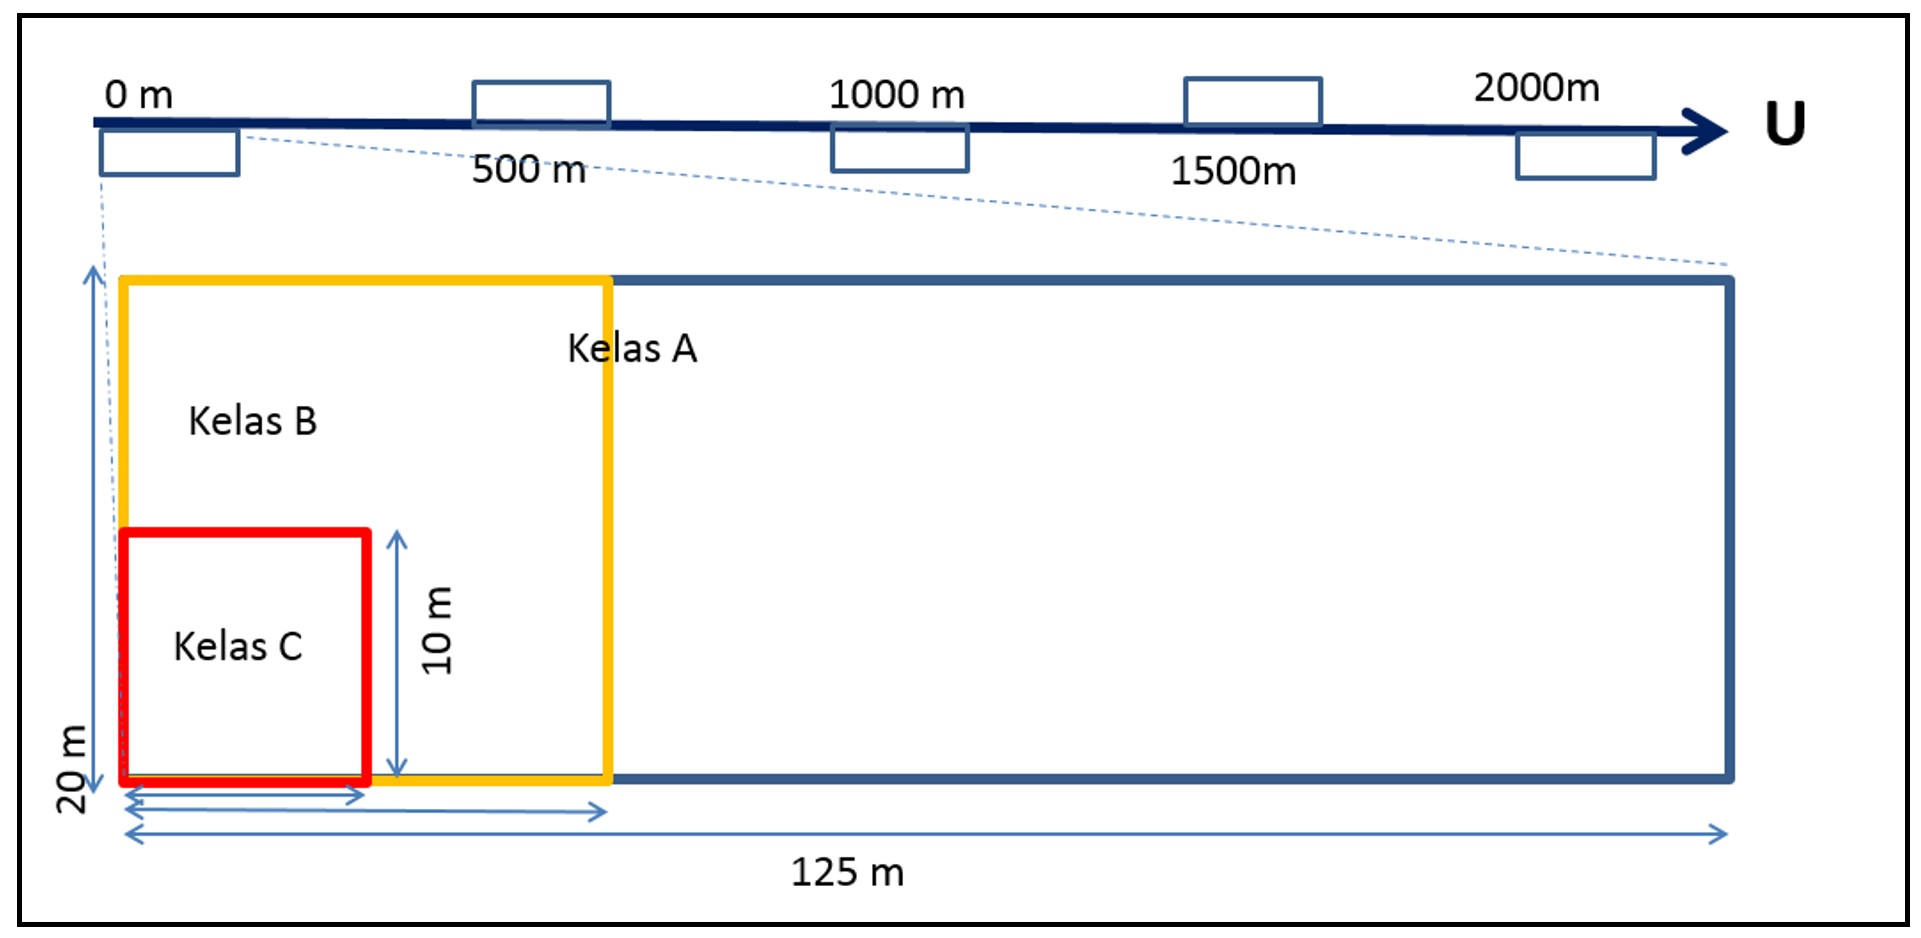
\includegraphics[width=1\linewidth]{images/pv_ilustration} 

}

\caption{Bentuk dan peletakan petak persegi terhadap jalur transek}\label{fig:figpv}
\end{figure}

\begin{longtable}[]{@{}
  >{\raggedright\arraybackslash}p{(\columnwidth - 2\tabcolsep) * \real{0.5000}}
  >{\raggedright\arraybackslash}p{(\columnwidth - 2\tabcolsep) * \real{0.5000}}@{}}
\caption{\label{tab:tabpvil} Teknik-teknik pengukuran diameter batang dengan kondisi khusus}\tabularnewline
\toprule()
\begin{minipage}[b]{\linewidth}\raggedright
Keterangan
\end{minipage} & \begin{minipage}[b]{\linewidth}\raggedright
Ilustrasi
\end{minipage} \\
\midrule()
\endfirsthead
\toprule()
\begin{minipage}[b]{\linewidth}\raggedright
Keterangan
\end{minipage} & \begin{minipage}[b]{\linewidth}\raggedright
Ilustrasi
\end{minipage} \\
\midrule()
\endhead
\textbf{Pohon di tanah yang miring.} Pengukuran diameter pohon di tanah yang miring dimulai dengan mengukur tinggi 1,3m dari permukaan tanah yang paling tinggi menyentuh dasar pohon. DBH dihitung pada bagian batang di titik 1,3m tersebut & 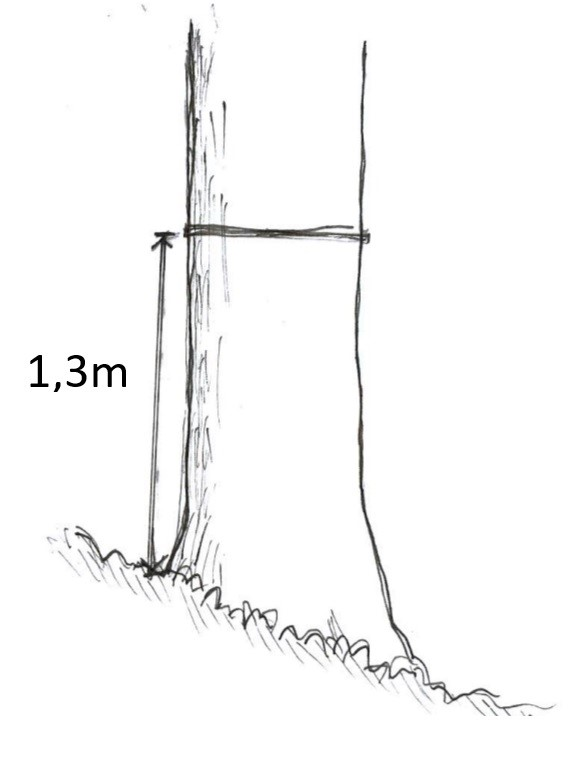
\includegraphics{images/vtb1.jpg} \\
\textbf{Pohon cacat (\emph{deform}) di titik 1,3 m.} Jika di titik 1,3m dari permukaan tanah, batang tidak bulat sempurna/cacat. maka titik pengukuran adalah pada 0,3m di atas dari ujung bagian yang cacat tersebut & 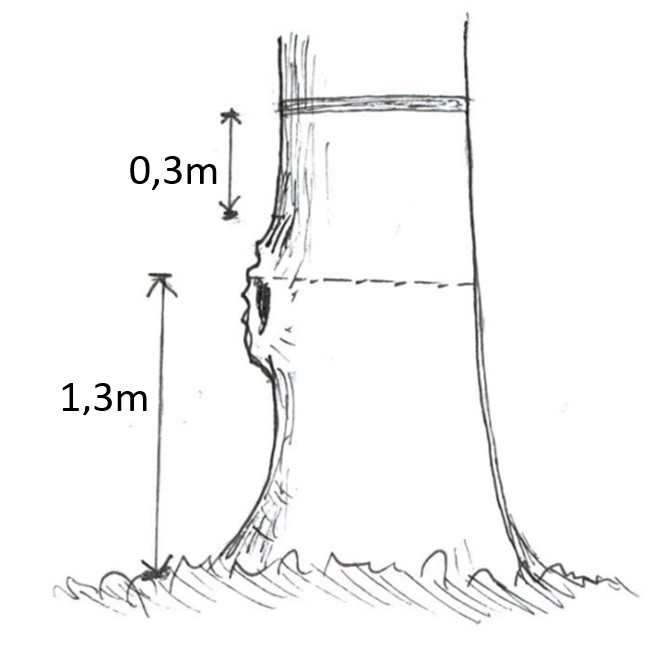
\includegraphics{images/vtb2.jpg} \\
\textbf{Pohon miring (leaning).} Pengukuran pada pohon miring dilakukan dengan mengukur 1,3m dari tanah pada sisi arah miring pohon tersebut/sisi yang terdekat dengan tanah & 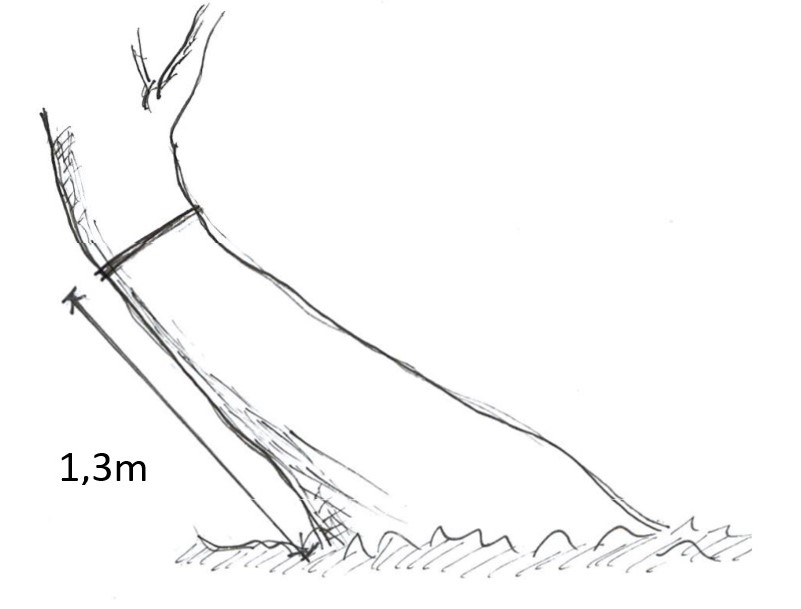
\includegraphics{images/vtb3.jpg} \\
\textbf{Pohon berbanir atau berakar tunjang.} jika tinggi banir atau akar tunjang di bawah 1,3m, maka pengukuran tetap dilakukan pada tinggi 1,3m & 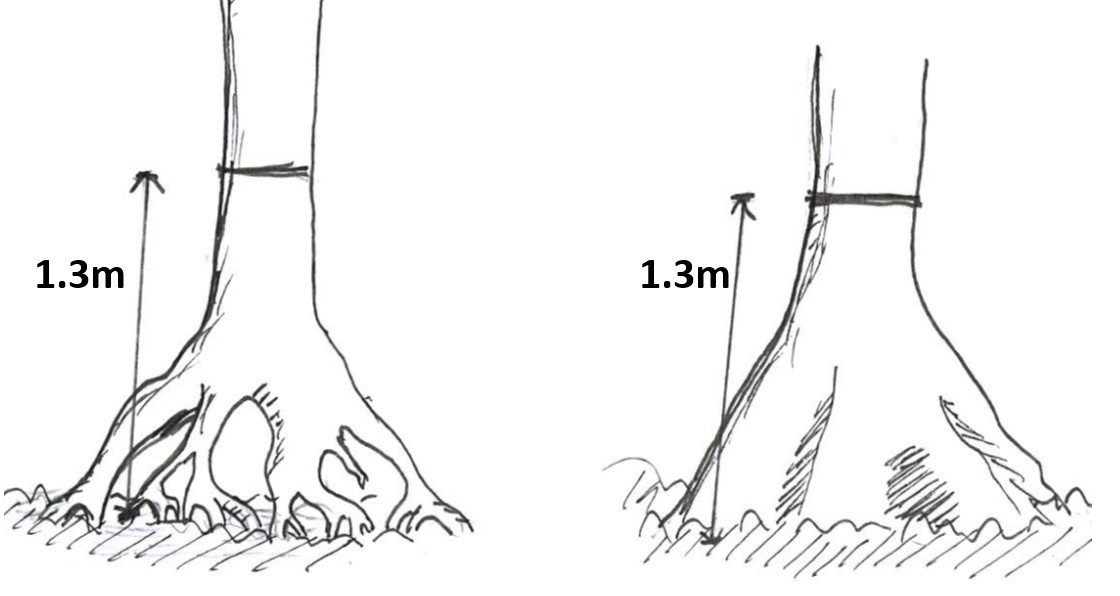
\includegraphics{images/vtb4.jpg} \\
Jika batas tinggi banir atau akar tunjang di atas 1,3 m dari permukaan tanah, maka pengukuran dilakukan di titik 0,3 m dari batas banir/akar tunjang & 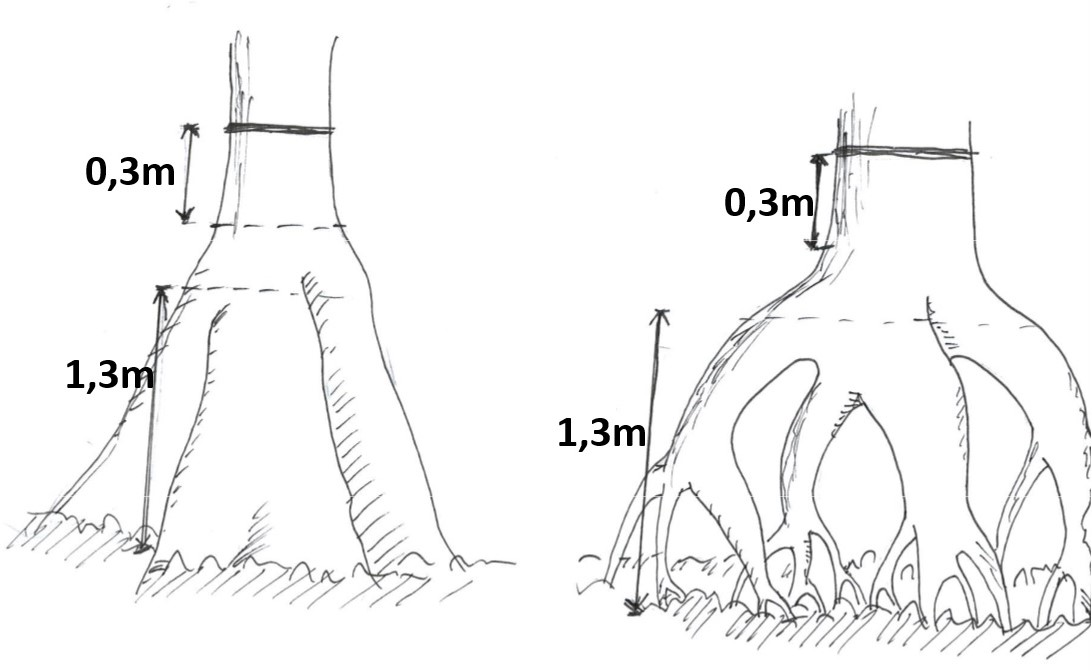
\includegraphics{images/vtb5.jpg} \\
Bila batas banir terlalu tinggi sehingga tidak memungkinkan untuk dipanjat, maka lakukan teknik dua tiang sesuai gambar di samping. Tiang didapat dari tegakan tingkat tiang lurus yang berasal dari luar petak dengan tinggi yang sesuai. Dua tiang disandingkan berjajar mengapit batang pada titik ukur diameter, orang ketiga memastikan bahwa tiang telah lurus, sejajar dan tepat di titik diameter, kemudian jarak antar tiang diukur dan dianggap sebagai diameter batang & 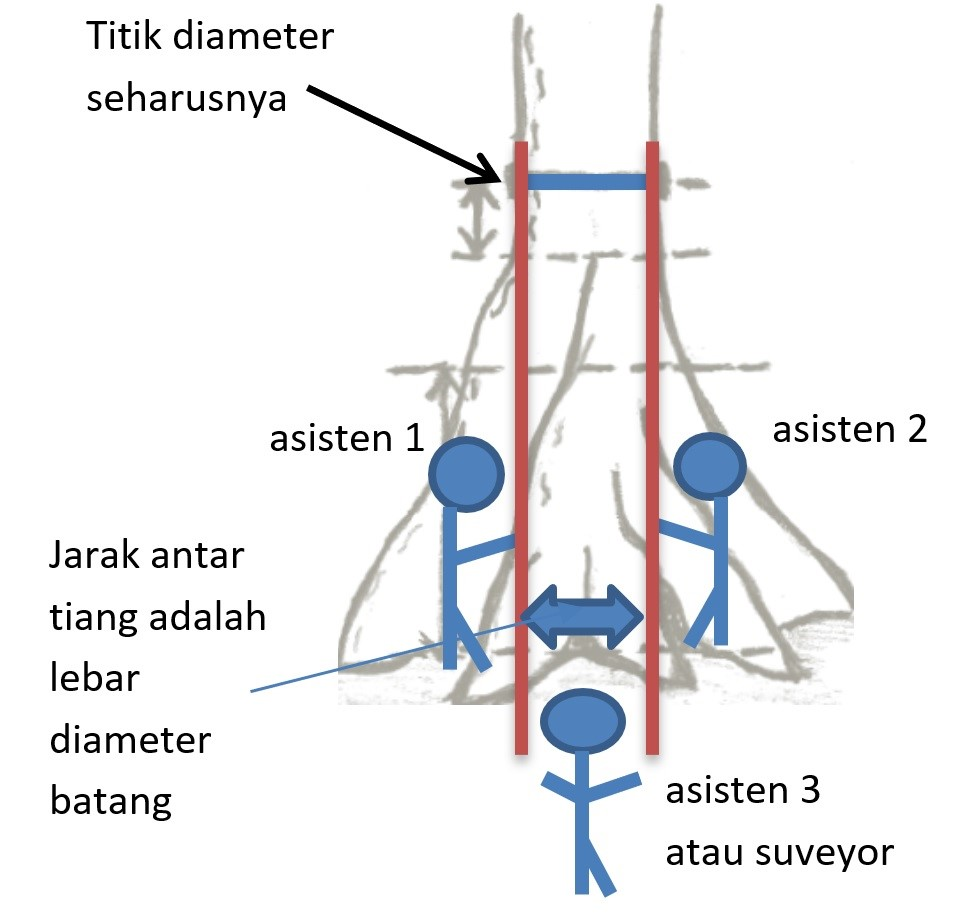
\includegraphics{images/vtb6.jpg} \\
\textbf{Pohon Bercabang atau Pohon berbatang ganda.} Jika pohon bercabang dengan tinggi cabang pada atau di atas 1,3m (a) maka pengukuran diameter dilakukan di bawah titik percabangan. Jika cabang pohon berada di bawah 1,3m (b), maka masing-masing batang diukur pada ketinggian 1,3 m dari permukaan tanah dan masing-masing cabang dianggap 1 tegakan & 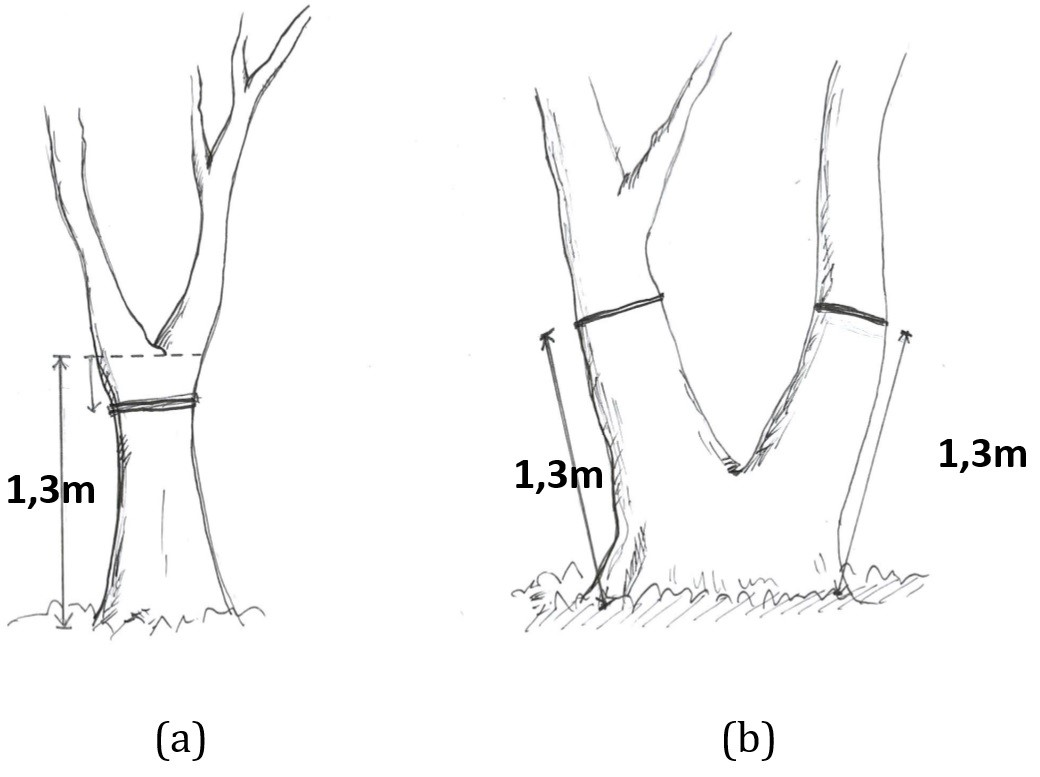
\includegraphics{images/vtb7.jpg} \\
\textbf{Pohon tumbang.} Pohon yang tumbang namun masih tumbuh dedaun hidup dianggap sebagai pohon hidup. Pengukuran diameter pohon ini dilakukan pada bagian batang sejauh 1,3m dari batas akar dan batang & 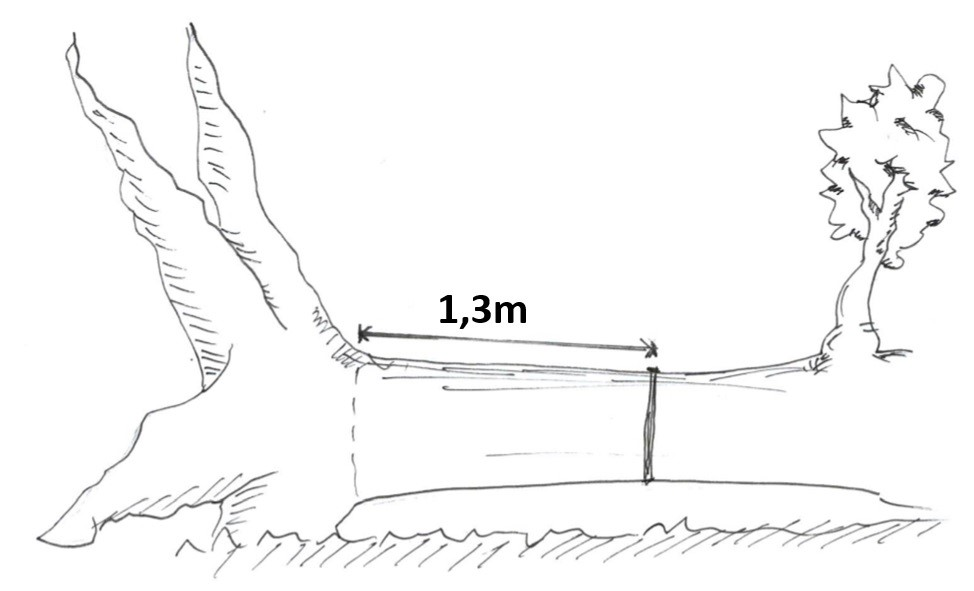
\includegraphics{images/vtb8.jpg} \\
\textbf{Pohon dengan liana.} Jika liana tumbuh pada titik pengukuran, jangan potong liana tersebut. Jika memungkinkan, Tarik liana menjauhi batang dan sematkan meter dbh tape di belakang liana sehingga dbh tape dapat melingkari batang dengan sempurna. Jika tidak memungkinkan, maka dengan bantuan pisau atau parang, buat dbh tape menyisip di antara liana sehingga dapat melingkari batang. Atau, jika liana sudah terlampau besar atau sudah sangat menempel pada batang, maka gunakan sisi belakang dari dbh tape (atau meteran ukur) untuk mengukur diameter batang secara visual & 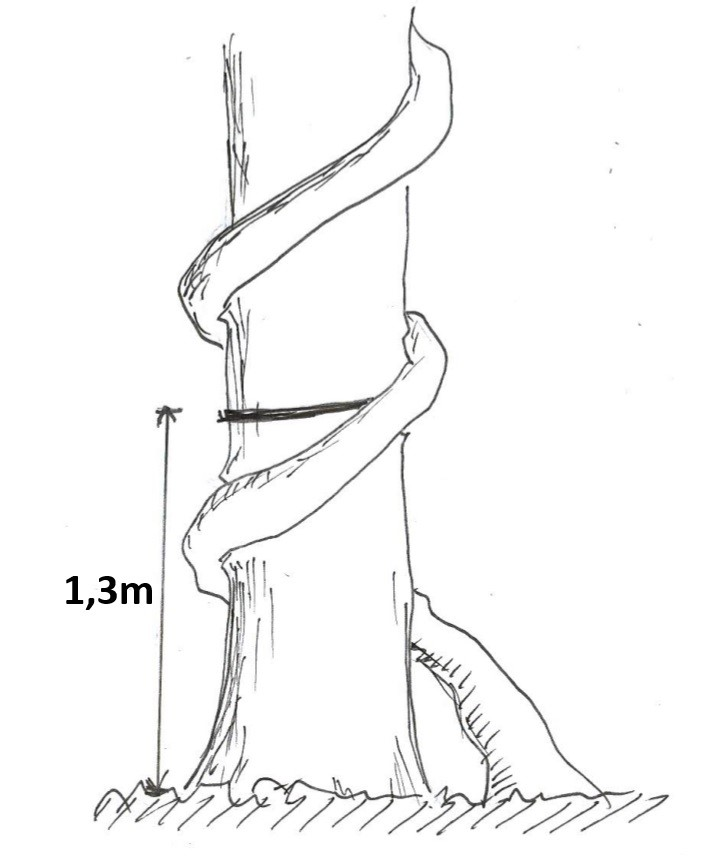
\includegraphics{images/vtb9.jpg} \\
\bottomrule()
\end{longtable}

\hypertarget{analisa-data}{%
\chapter*{Analisa Data}\label{analisa-data}}
\addcontentsline{toc}{chapter}{Analisa Data}

\hypertarget{pengelolaan-data}{%
\chapter*{Pengelolaan Data}\label{pengelolaan-data}}
\addcontentsline{toc}{chapter}{Pengelolaan Data}

\hypertarget{lampiran-1.-lembar-data}{%
\chapter*{Lampiran 1. Lembar Data}\label{lampiran-1.-lembar-data}}
\addcontentsline{toc}{chapter}{Lampiran 1. Lembar Data}

Peran lembar data dalam kajian survei kehati sangat penting. Penggunaan lembar data yang tepat membuat pencatatan temuan menjadi lebih efisien dan terstandarisasi. Dalam lampiran ini terlampir contoh-contoh lembar data untuk setiap taksa. Templat lembar data tersedia pada tautan ini: \emph{Tallysheet-biodive}. Pembaca bisa mengunduh dan memperbanyak lembar data sebanyak yang dibutuhkan sebelum survei. Pada praktiknya, mungkin lembar data yang penulis sediakan belum mencakup hal spesifik yang dibutuhkan oleh projek, oleh karena itu pembaca bisa menambahkan sendiri kolom-kolom yang dibutuhkan.

Selalu gunakan pensil dalam menulis di lembar data dan jika memungkinkan gunakan kertas tahan air, karena kemungkinan basah karena hujan sangat tinggi. Setelah selesai dari lapang, harus langsung dipindai untuk disimpan sebagai salinan digital. Lembar data yang ditulis dilapangan ini merupakan data primer untuk verifikasi seandainya ada kesalahan input saat surveior memindahkan ke dalam excel.

\hypertarget{lembar-data-avifauna}{%
\section*{Lembar Data Avifauna}\label{lembar-data-avifauna}}
\addcontentsline{toc}{section}{Lembar Data Avifauna}

\textbf{Lembar data pengamatan menggunakan titik hitung}

Pada awal lembar data dibutuhkan informasi umum mengenai tanggal, lokasi, durasi pengamatan, dan seluruh personil yang terlibat. Untuk lokasi geografis dari GPS, set menjadi decimal degree supaya bisa konsisten diseluruh Indonesia dan mudah di-input ke dalam sistem computer (Excel, dll). Keterangan dari setiap kolom adalah sebagai berikut;

\textbf{Jenis:} Nama jenis burung menggunakan nama latin, namun apabila belum mengetahui jenisnya, dapat menggunakan nama lokal terlebih dahulu.

\textbf{Individu:} Jumlah burung yang ditemukan pada satu spot (beberapa burung terkadang berkelompok atau berpasangan seperti cendrawasih atau burung gereja)

\textbf{Jarak:} Jarak burung dari pengamat dalam satuan meter

\textbf{Catatan:} Tambahan catatan penting jika ada

\begin{figure}

{\centering 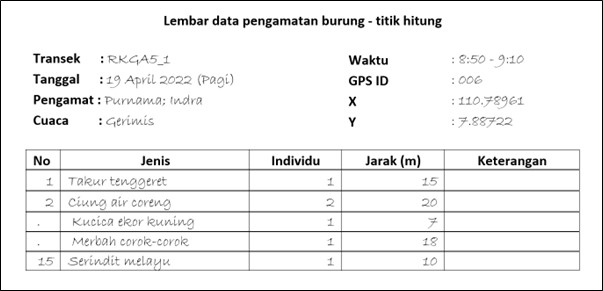
\includegraphics[width=1\linewidth]{images/ldp_th} 

}

\caption{Contoh lembar data untuk metode titik hitung}\label{fig:ldpth}
\end{figure}

\textbf{Lembar data parameter lingkungan di titik hitung}

Dalam setiap titik hitung, dapat ditambahkan parameter lingkungan untuk melihat pengaruh perbedaan rona lingkungan terhadap komunitas burung, Adapun keterangan dari setiap baris adalah sebagai berikut

\textbf{Tallest tree (m):} Pohon tertinggi disekitar lokasi pengamatan. Satuan nilai dalam meter

\textbf{Ground cover (\%):} Tutupan bawah disekitar lokasi pengamatan satuan nilai (\%)

\textbf{Plant height 0-1,5 m (\%):} Jumlah persentase pohon dengan ukuran 0-1.5 m disekitar lokasi pengamatan

\textbf{Plant height 1,5-5 m (\%):} Jumlah persentase pohon dengan ukuran 1.5-5 m disekitar lokasi pengamatan

\textbf{Plant height 5-15 m (\%):} Jumlah persentase pohon dengan ukuran 5-15 m disekitar lokasi pengamatan

\textbf{Plant height \textgreater15 m (\%):} Jumlah persentase pohon dengan ukuran \textgreater15 m disekitar lokasi pengamatan

\textbf{Bole climb (\%):} Persentase tumbuhan yang merambat disekitar lokasi pengamatan

\textbf{Liana (\%):} Persentase tumbuhan pemanjat disekitar lokasi pengamatan

\textbf{Macaranga (\%):} Persentase tumbuhan jenis macaranga disekitar lokasi pengamatan

\textbf{Rattan (\%):} Persentase rotan disekitar lokasi pengamatan

\textbf{Fern (\%):} Persentase paku-pakuan disekitar lokasi pengamatan

\textbf{Small palm (\%):} Persentase palem-paleman disekitar lokasi pengamatan

\textbf{Dist. from water:} Kategori jarak ke sumber air; 1 = 0-50 m, 2 = 50-100m, 3 \textgreater{} 100m

\textbf{Logs abd:} Jumlah pohon tumbang yang ada dilokasi pengamatan

\textbf{Snags abd:} Jumlah pohon mati berdiri disekitar lokasi pengamatan

\textbf{Zingiberaceae (\%):} Persentase temu-temuan/rimpang disekitar lokasi pengamatan

\textbf{Grass (\%):} Persentase rumput-rumputan disekitar lokasi pengamatan

\textbf{Moss (cm):} Ketebalan lumut disekitar lokasi pengamatan dalam centimeter

\textbf{Litter (cm):} Ketebalan seresah disekitar lokasi pengamatan dalam centimeter

\begin{figure}

{\centering 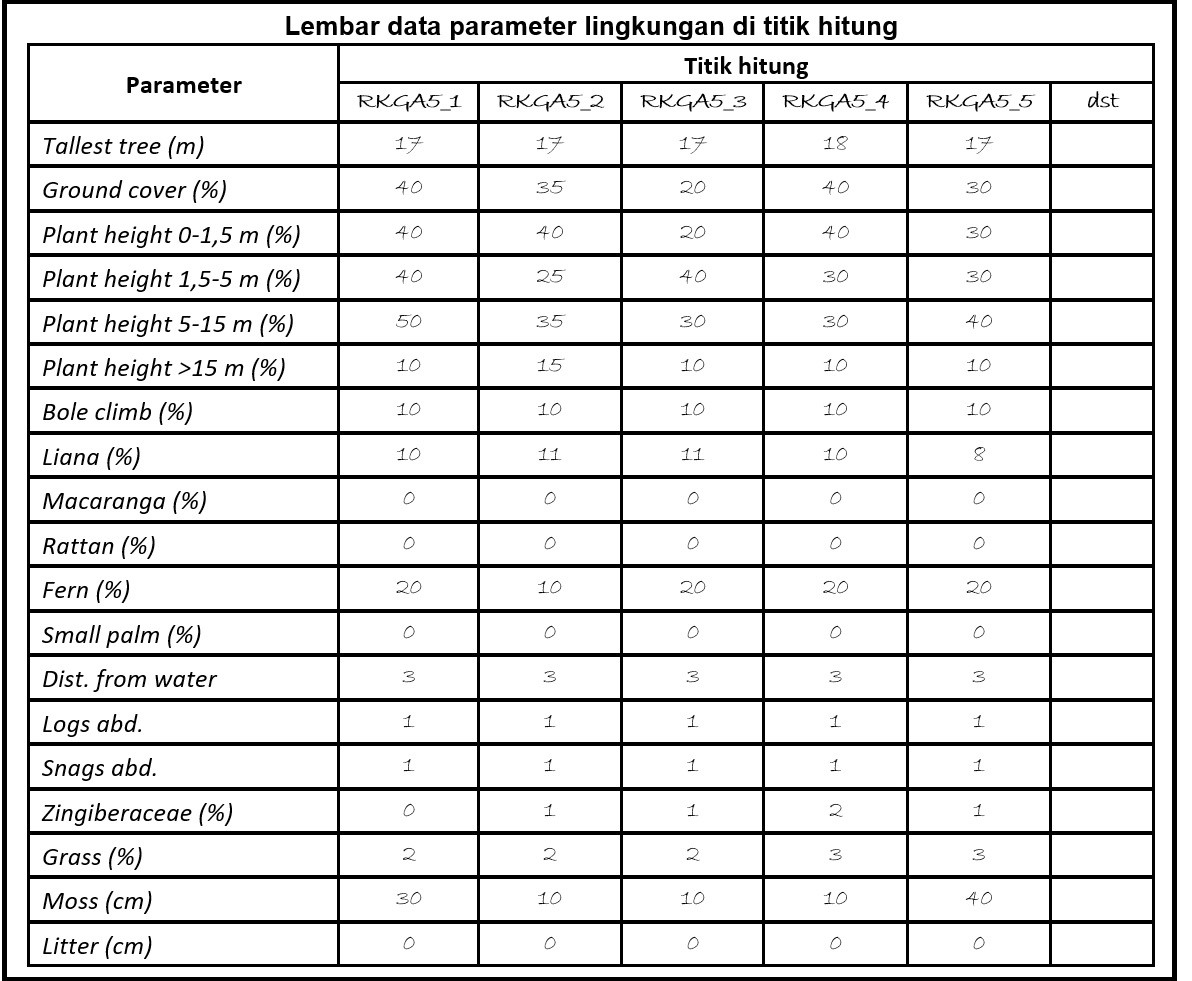
\includegraphics[width=1\linewidth]{images/ldp_pl} 

}

\caption{Contoh lembar data untuk parameter lingkungan di setiap titik hitung}\label{fig:ldppl}
\end{figure}

\textbf{Lembar data daftar jenis MacKinnon}

Pada pengamatan yang bersifat ekploratif menggunakan daftar jenis MacKinnon, lembar data yang digunakan sangat sederhana, dengan diawali informasi pengamat, lokasi dan durasi pengamatan

\begin{figure}

{\centering 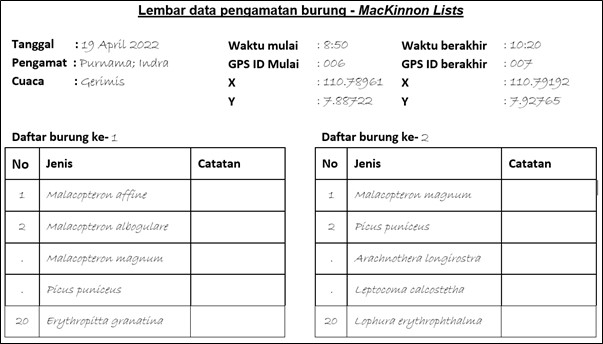
\includegraphics[width=1\linewidth]{images/ldp_ml} 

}

\caption{Contoh lembar data untuk daftar jenis MacKinnon}\label{fig:ldpml}
\end{figure}

\hypertarget{lembar-data-herpetofauna}{%
\section*{Lembar Data Herpetofauna}\label{lembar-data-herpetofauna}}
\addcontentsline{toc}{section}{Lembar Data Herpetofauna}

\textbf{Lembar data pengamatan menggunakan metode \emph{VES}}

Pada awal lembar data dibutuhkan informasi umum mengenai tanggal, lokasi, durasi pengamatan, dan seluruh personil yang terlibat. Untuk lokasi geografis dari GPS, set menjadi decimal degree supaya bisa konsisten diseluruh Indonesia dan mudah di-input ke dalam sistem computer (Excel, dll). Keterangan dari setiap kolom adalah sebagai berikut;

\textbf{Waktu:} Jam ditemukannya herpetofauna, gunakan format hh;mm (0:00 -- 24:00)

\textbf{Jenis:} Nama jenis menggunakan nama latin, namun apabila belum mengetahui jenisnya, dapat menggunakan nama lokal terlebih dahulu.

\textbf{SVL (cm):} Panjang tubuh dari moncong hingga pangkal ekor dalam satuan cm

\textbf{Hor (m):} (a) survei di sempadan sungai; jarak horisontal dari sungai (b) survei di transek; jarak horisontal dari garis tengah transek

\textbf{Ver (m):} (a) survei di sempadan sungai; Jarak vertikal dari badan air (b) survei di transek; jarak vertikal dari permukaan tanah

\textbf{Substrat:} Substrat atau pijakan dari satwa yang ditemukan

\textbf{Aktivitas:} Aktivitas spesifik pada saat ditemukan

\begin{figure}

{\centering 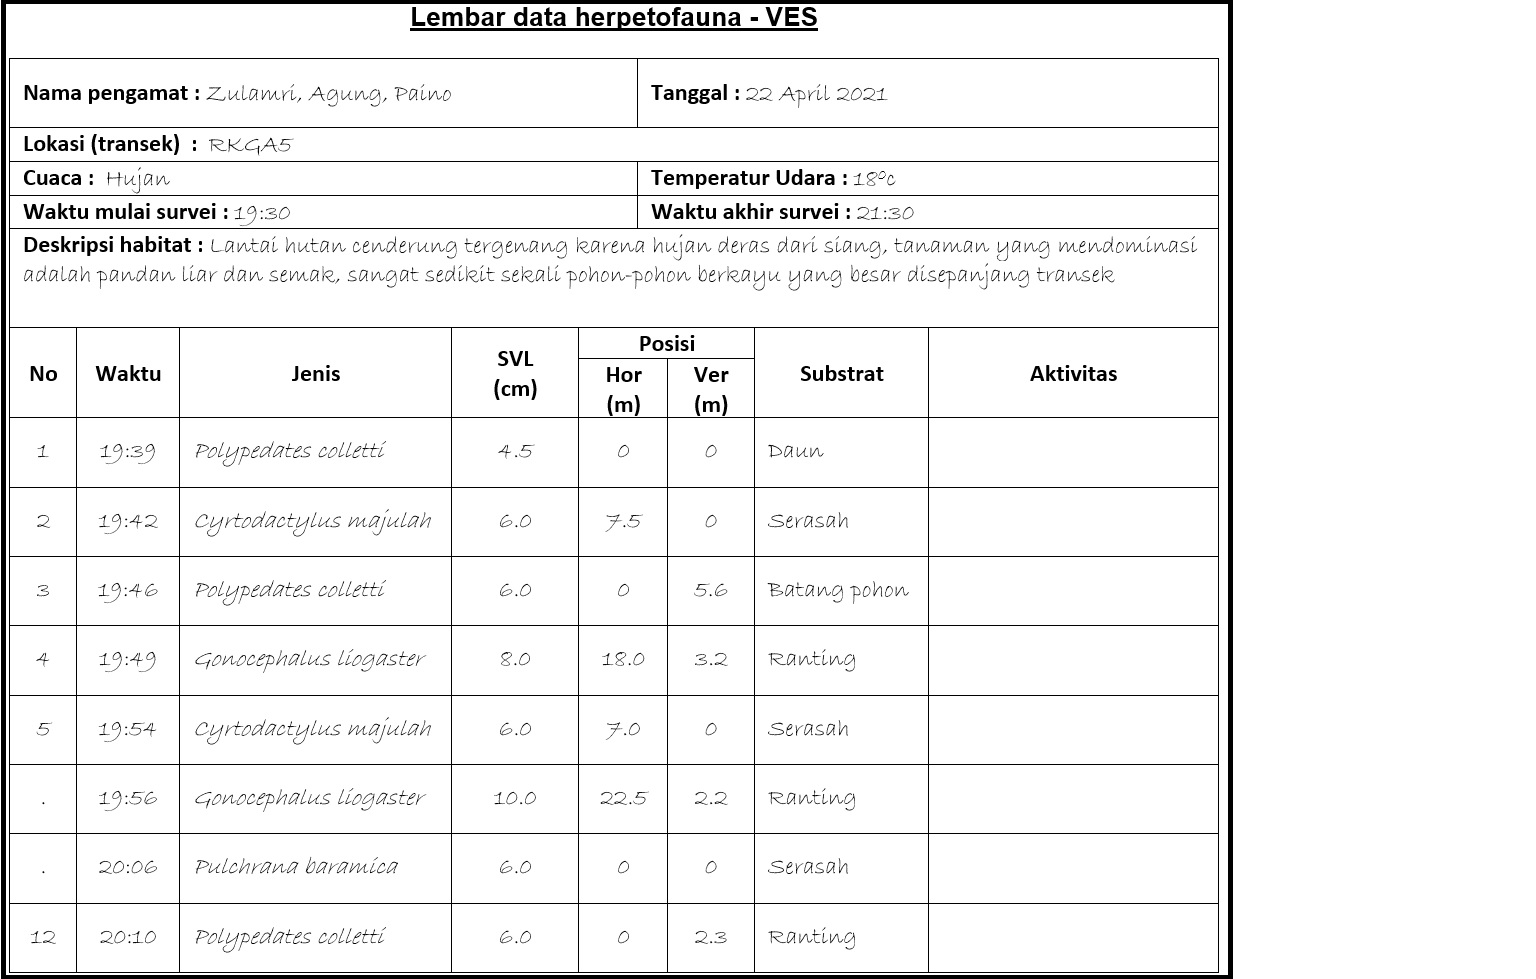
\includegraphics[width=1\linewidth]{images/ldh_ves} 

}

\caption{Contoh lembar data untuk metode VES}\label{fig:ldhves}
\end{figure}

\hypertarget{lembar-data-mamalia}{%
\section*{Lembar Data Mamalia}\label{lembar-data-mamalia}}
\addcontentsline{toc}{section}{Lembar Data Mamalia}

\textbf{Lembar data pengamatan menggunakan transek garis dan eksplorasi}

Pada awal lembar data dibutuhkan informasi umum mengenai tanggal, lokasi, durasi pengamatan, dan seluruh personil yang terlibat. Untuk lokasi geografis dari GPS, set menjadi decimal degree supaya bisa konsisten diseluruh Indonesia dan mudah di-input ke dalam sistem computer (Excel, dll). Keterangan dari setiap kolom adalah sebagai berikut;

\textbf{Waktu:} Jam ditemukannya mamalia, gunakan format hh;mm (0:00 -- 24:00)

\textbf{Jenis:} Nama jenis menggunakan nama latin, namun apabila belum mengetahui jenisnya, dapat menggunakan nama lokal terlebih dahulu.

\textbf{PPD (M):} Jarak perpendicular satwa ditemukan pertama kali, relatif terhadap garis tengah transek jika memungkinkan.

\textbf{Tipe temuan:} Tipe temuan satwa dapat diisi dengan perjumpaan langsung, kotoran, cakaran, maupun suara. Pembeda temuan ini untuk mengukur akurasi identifikasi.

\textbf{GPS ID:} Nomor waypoint pada GPS. Supaya survei lebih efisien, pengamat boleh menulis nomor waypoint pada GPS terlebih dahulu selama pengamatan, untuk kemudian melengkapi koordinat pada saat sudah di kamp.

\textbf{Lon:} Lokasi koordinat Longitude (X). Referensi kordinat yang dipakai adalah WGS84 dengan format penulisan decimal degree.

\textbf{Lat:} Lokasi koordinat Latitude (Y). Referensi kordinat yang dipakai adalah WGS84 dengan format penulisan decimal degree.

\textbf{Catatan:} Tambahkan catatan penting jika ada

\begin{figure}

{\centering 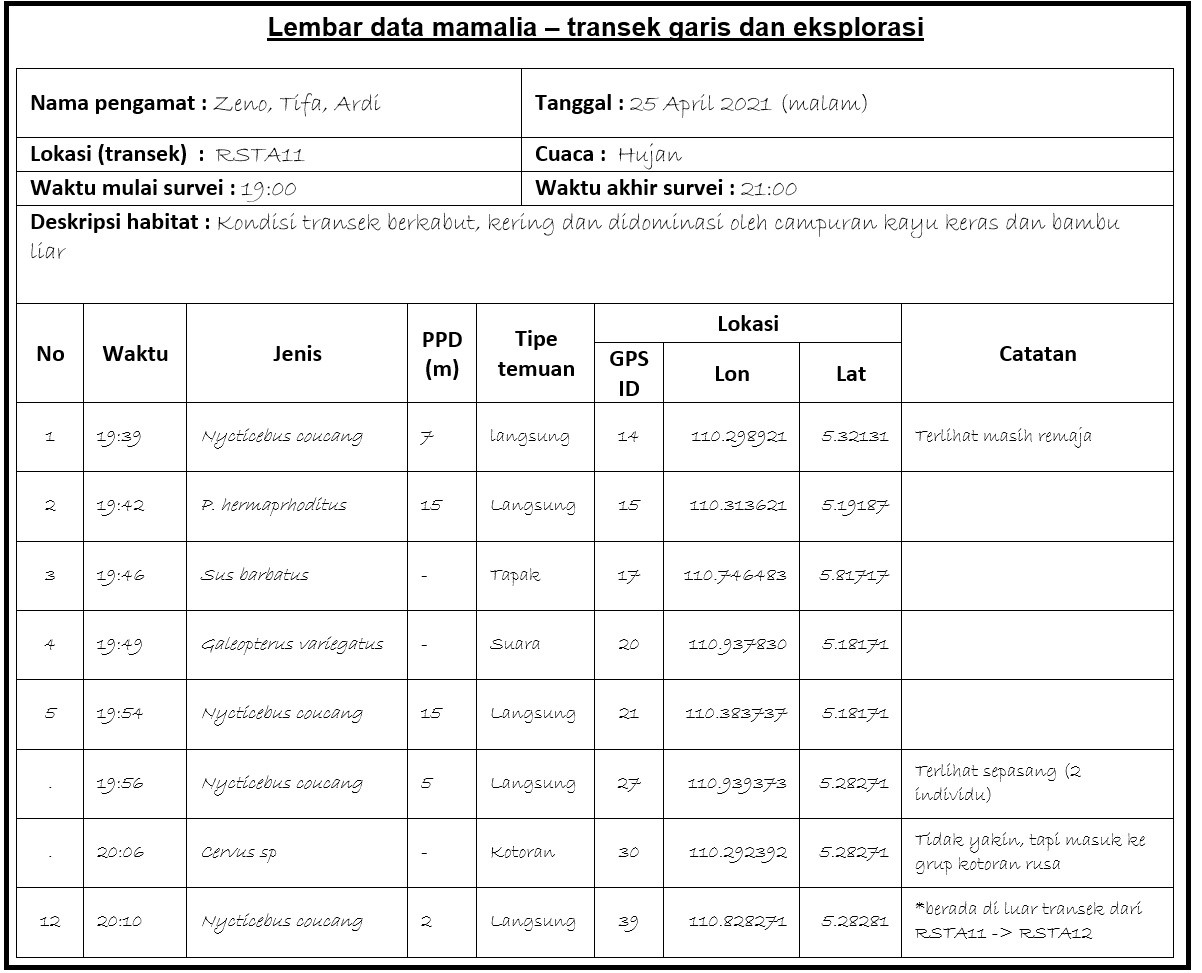
\includegraphics[width=1\linewidth]{images/ldm_tg} 

}

\caption{Contoh lembar data untuk metode transek garis}\label{fig:ldmtg}
\end{figure}

\textbf{Lembar data pengamatan mamalia kecil menggunakan perangkap}

Khusus untuk pengamatan mamalia kecil menggunakan perangkap, menggunakan contoh lembar data dan keterangan di bawah ini. Lembar data ini terdiri dari dua bagian, dimana bagian kedua berisi informasi perangkap yang digunakan pada bagian selanjutnya untuk dapat mengukur usaha survei dan informasi lokasi disetiap perangkap.

\textbf{Tanggal:} Tanggal ditemukan satwa

\textbf{Waktu:} Jam ditemukan satwa

\textbf{Trap ID:} Nomor unik setiap perangkap yang digunakan

\textbf{Jenis:} Nama jenis menggunakan nama latin, namun apabila belum mengetahui jenisnya, dapat menggunakan nama lokal terlebih dahulu.

\textbf{Usia:} kriteria usia satwa jika diketahui

\textbf{Sex:} Jenis kelamin satwa jika diketahui

\textbf{HB (mm):} Panjang tubuh satwa dalam satuan milimeter

\textbf{FA (mm):} Panjang lengan atau kaki depan satwa dalam sattuan milimeter

\textbf{E (mm):} Panjang telinga satwa

\textbf{T (mm):} Panjang ekor satwa

\textbf{HF (mm): }Panjang kaki belakang satwa

\textbf{W (gr):} Berat tubuh satwa dalam gram

\textbf{AT (mm): }Panjang anti tragus dalam milimeter, khusus untuk satwa kelelawar

\textbf{TR (mm):} Panjang tragus dalam milimeter, khusus untuk satwa kelelawar

\textbf{Catatan: }Tambahan catatan penting jika ada

\begin{figure}

{\centering 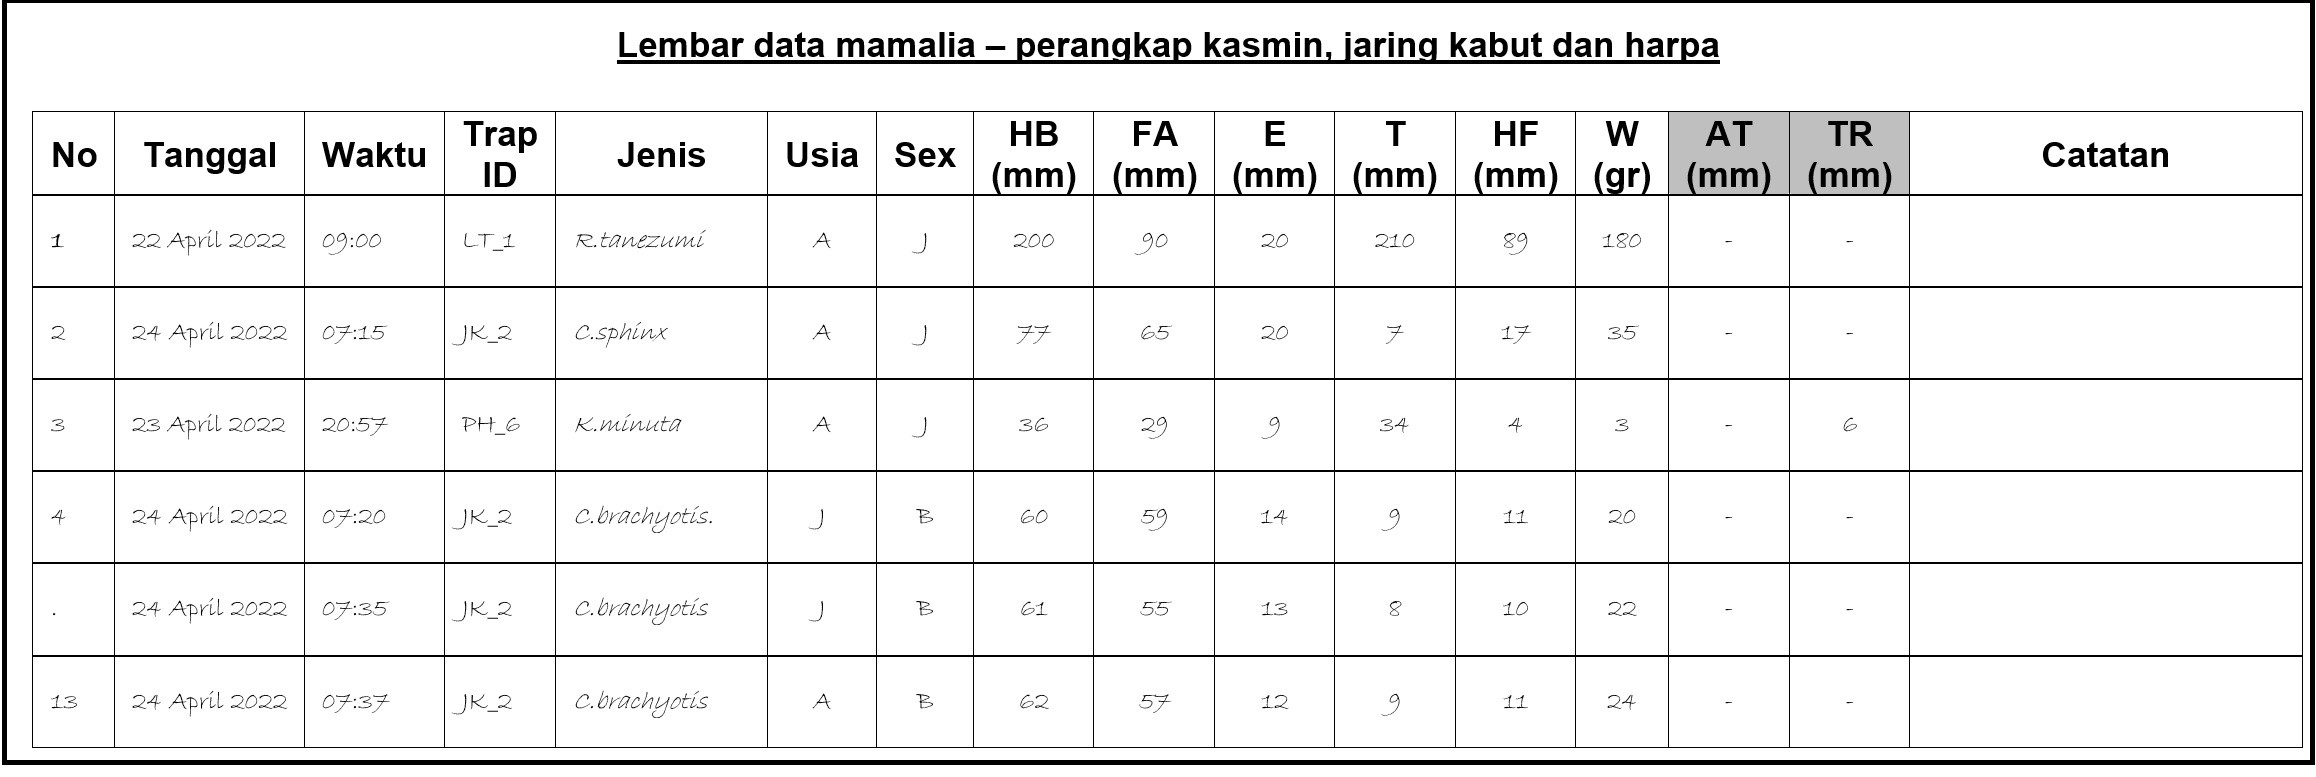
\includegraphics[width=1\linewidth]{images/ldm_pk} 

}

\caption{Contoh lembar data untuk pengamatan menggunakan perangkap}\label{fig:ldmpk}
\end{figure}

\textbf{Lembar data informasi perangkap yang digunakan}

Lembar data dibawah ini merupakan bagian kedua yang berisi informasi seluruh perangkap selama melakukan kajian. Lembar data ini merupakan bagian kedua dari lembar data sebelumnya, dengan informasi setiap kolom sebagai berikut;

\textbf{Trap ID:} Nomor unik setiap perangkap yang digunakan

\textbf{Tipe:} Tipe atau jenis perangkap yang digunakan

\textbf{GPS ID:} Nomor waypoint pada GPS. Supaya survei lebih efisien, pengamat boleh menulis nomor waypoint pada GPS terlebih dahulu selama pengamatan, untuk kemudian melengkapi koordinat pada saat sudah di kamp.

\textbf{Lon:} Lokasi koordinat Longitude (X). Referensi kordinat yang dipakai adalah WGS84 dengan format penulisan decimal degree.

\textbf{Lat:} Lokasi koordinat Latitude (Y). Referensi kordinat yang dipakai adalah WGS84 dengan format penulisan decimal degree.

\textbf{Tanggal pasang:} Tanggal perangkap mulai dipasang atau diaktifkan

\textbf{Tangggal selesai:} Tanggal perangkap selesai digunakan

\textbf{Waktu pasang:} Waktu mulai perangkap dipasang atau diaktifkan

\textbf{Waktu selesai:} waktu berakhirnya perangkap digunakan

\textbf{Catatan:} Tambahan catatan penting jika ada

\begin{figure}

{\centering 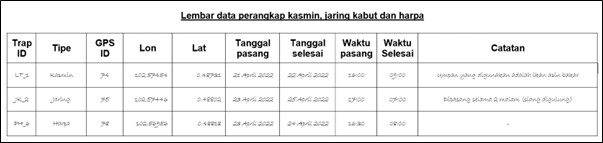
\includegraphics[width=1\linewidth]{images/ldm_p} 

}

\caption{Contoh lembar data informasi perangkap}\label{fig:ldmp}
\end{figure}

\hypertarget{lembar-data-vegetasi}{%
\section*{Lembar Data Vegetasi}\label{lembar-data-vegetasi}}
\addcontentsline{toc}{section}{Lembar Data Vegetasi}

\textbf{Lembar data informasi petak vegetasi}

Lembar data vegetasi memiliki dua bagian utama. Bagian pertama berisi mengenai informasi personil, lokasi referensi geografis, dan keadaan umum disekitar plot dengan contoh dan informasi dibawah ini;

\textbf{Nomor ID Plot:} Nomor unik plot

\textbf{Koordinat GPS (X):} Lokasi koordinat Longitude (X). Referensi kordinat yang dipakai adalah WGS84 dengan format penulisan decimal degree.

\textbf{Koordinat GPS (Y):} Lokasi koordinat Latitude (Y). Referensi kordinat yang dipakai adalah WGS84 dengan format penulisan decimal degree.

\textbf{Arah plot:} arah plot (barat, timur, utara, selatan)

\textbf{Waktu (tanggal, jam):} informasi waktu dan jam memulai pengamatan di plot

\textbf{Cuaca:} cuaca pada saat pengamatan

\textbf{Substrat:} Kondisi subsrat dominan yang ada di plot

\textbf{Anggota tim:} nama-nama seluruh personil

\textbf{Tipe habitat:} Kondisi deksriptif habitat atau vegetasi yang dominan di plot

\textbf{Drainase lantai hutan:} Kondisi lantai hutan, tandai dengan silang pilihan yang ada disebelah kanannya

\textbf{Gangguan:} Gangguan atau potensi gangguan yang ada di dalam dan sekitar plot

\textbf{Nomor foto rona vegetasi:} nomor foto yang ada di kamera, mengenai foto-foto rona vegetasi yang ada di dalam plot

\textbf{Catatan tambahan:} Catatan tambahan jika diperlukan mengenai kondisi plot.

\begin{figure}

{\centering 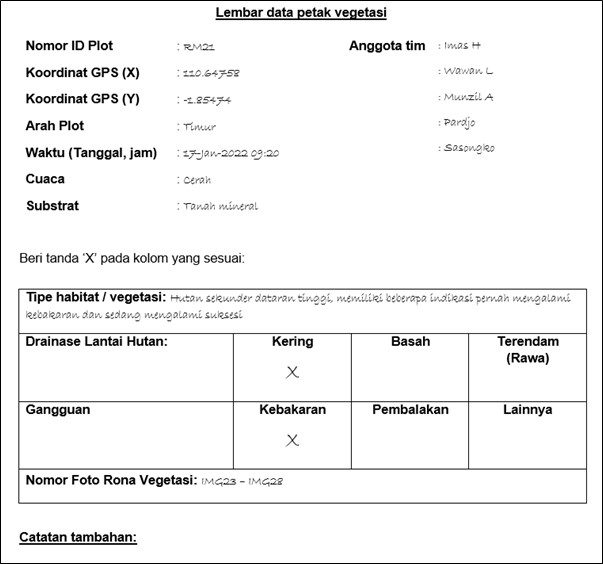
\includegraphics[width=1\linewidth]{images/ldv_ip} 

}

\caption{Contoh lembar data petak vegetasi}\label{fig:ldvip}
\end{figure}

\textbf{Lembar data vegetasi}

Lembar data ini merupakan bagian kedua dari set lembar data vegetasi untuk menulis pengukuran tumbuhan di setiap anak petak dengan contoh dan informasi setiap kolom sebagai berikut;

\textbf{Kelas:} Kelas kategori tumbuhan berdasarkan ukuran diameter batang

\textbf{Jenis:} Nama jenis menggunakan nama latin, namun apabila belum mengetahui jenisnya, dapat menggunakan nama lokal terlebih dahulu.

\textbf{Kode pohon:} Kode penanda individu tumbuhan didalam plot

\textbf{DBH (cm):} Diameter batang setinggi dada (Dbh) dalam satuan cm

\textbf{TT (m):} Tinggi total tanaman dalam meter

\textbf{TBC (m):} Tinggi bebas cabang dalam satuan meter

\textbf{Kode foto:} Nomor foto di kamera
\textbf{Keterangan:} Catatan atau keterangan tambahan jika diperlukan

\begin{figure}

{\centering 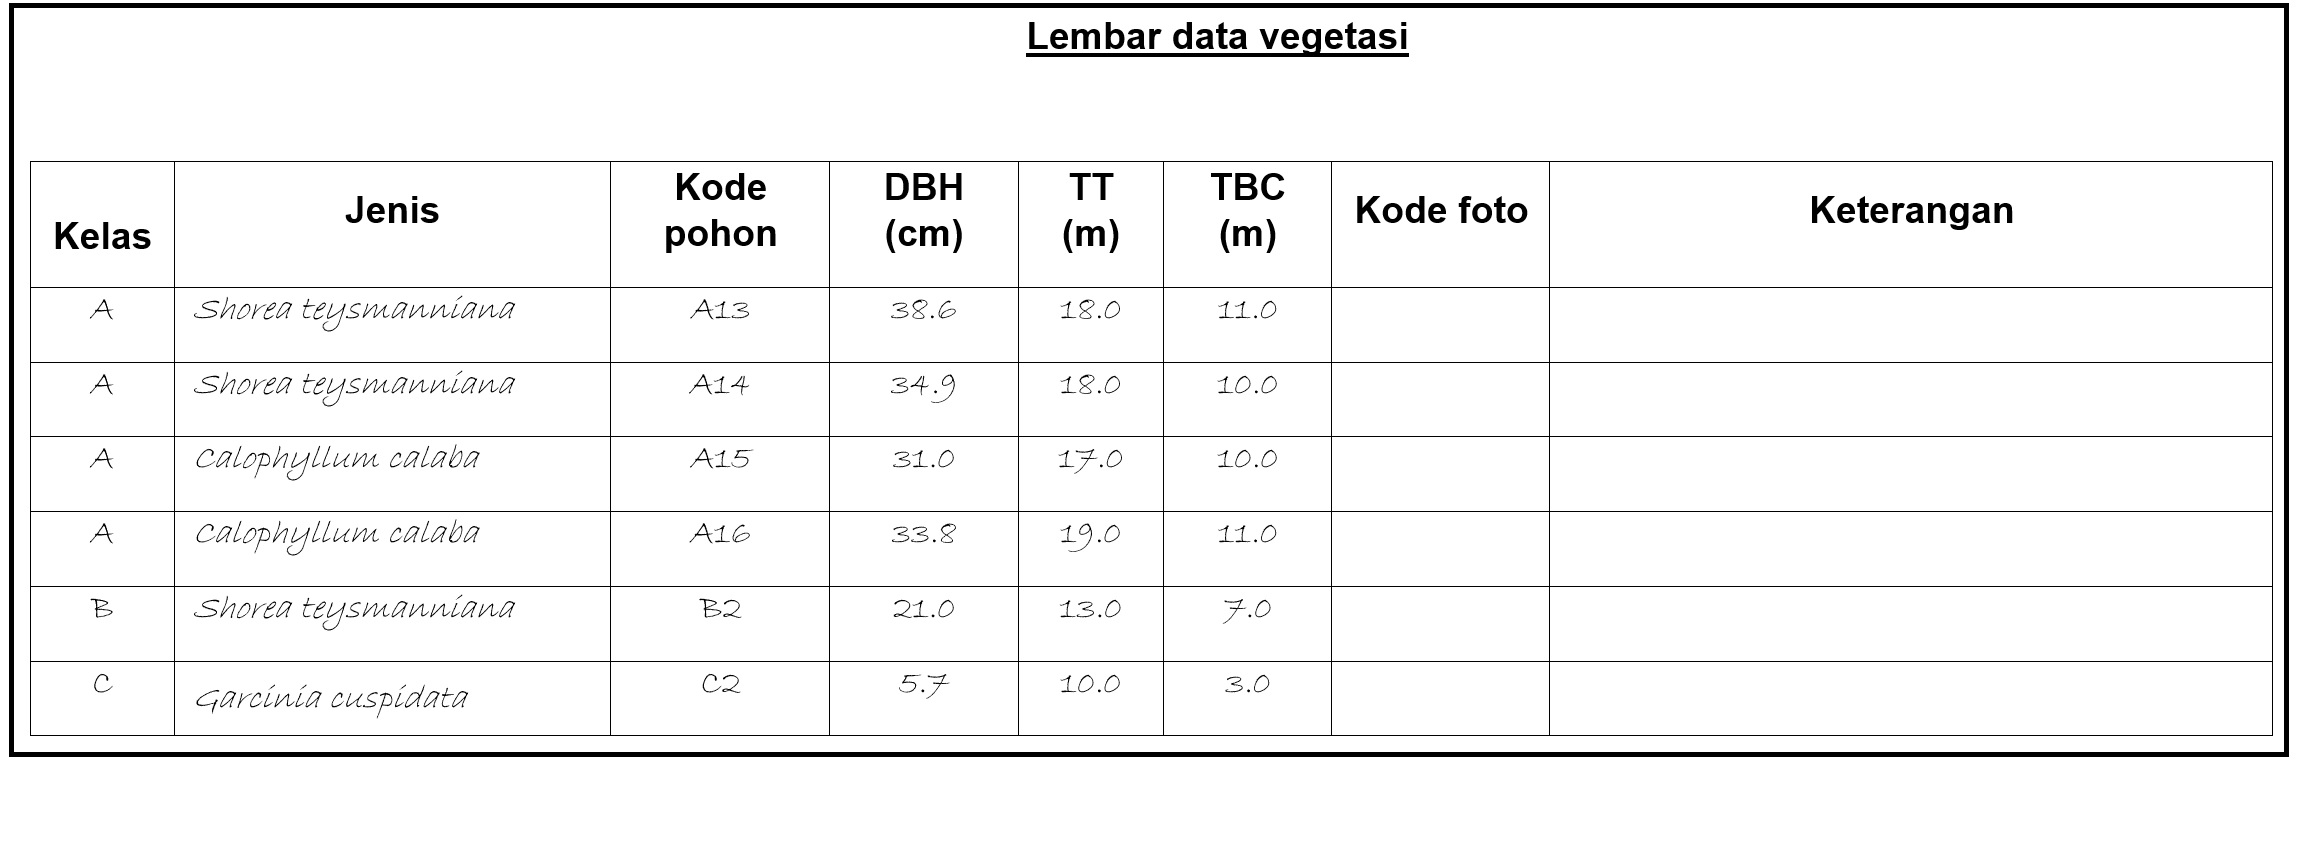
\includegraphics[width=1\linewidth]{images/ldv_m} 

}

\caption{Contoh lembar data vegetasi}\label{fig:ldvm}
\end{figure}

\end{document}
